\section{Konzeption und prototypische Umsetzung}
\subsection{Anforderungen}
Die Anforderungen an die Schnittstelle und den daraus resultierenden Prototyp wurden in Zusammenarbeit mit CONET erhoben. Die Projektidee entstand im Kontext eines Projektes zu Trendscouting-Systemen. Das Ziel des Systems sollte es sein, eine Architektur bereitzustellen, die vom Nutzer gestellte Anfragen annimmt und diese mit einer KI analysiert, um Aussagen darüber treffen zu können, welche Technologien in der Zukunft relevant werden könnten. Aus dieser Projektidee ergab sich als Zielsetzung die Entwicklung einer Architektur, die ein solches System unterstützen könnte. Die genaue Anforderungserhebung wurde nach dem Leitfaden der von der \ac{iec} veröffentlichten Norm IEC 62304 Kapitel 5.2 entworfen.\footcite{daniel2018anforderungen} Diese Norm spezifiziert, wie Anforderungen an eine Software aufbereitet und dokumentiert werden sollen.

Auf der Grundlage dieser Norm wurden die Benutzerschnittstellen für den Prototyp spezifiziert. Die grundlegende Interaktion mit dem System findet über die Website statt. Dort hat der Nutzer die Möglichkeit, seine Suchanfrage in Form eines ausgeschriebenen Satzes oder über einzelne Stichpunkte in ein Textfeld einzugeben. Die nächste Benutzerschnittstelle ist die Transformation der zuvor eingegebenen Suchanfrage. Der Nutzer soll dort mittels JSON-Syntax die Suchanfrage modifizieren können. Dies ist im Hinblick auf eine eventuell automatisierte Nutzung des Systems erforderlich. Im dritten Schritt soll der Nutzer die Option haben, die Suchparameter für die KI anzupassen. Insbesondere   die Anzahl der Ergebnisse ist relevant, die bei einer gestellten Suchanfrage zurückgegeben werden. An dieser Stelle sollen auch weitere Parameter eingegeben werden können. Anschließend ist eine Möglichkeit vorgesehen die Anfrage inklusive der Parameter abzuschicken. Abbildung 5 stellt die Interaktion mit dem System in einem Use-Case-Diagramm dar.

\begin{figure}[H]
  \centering
    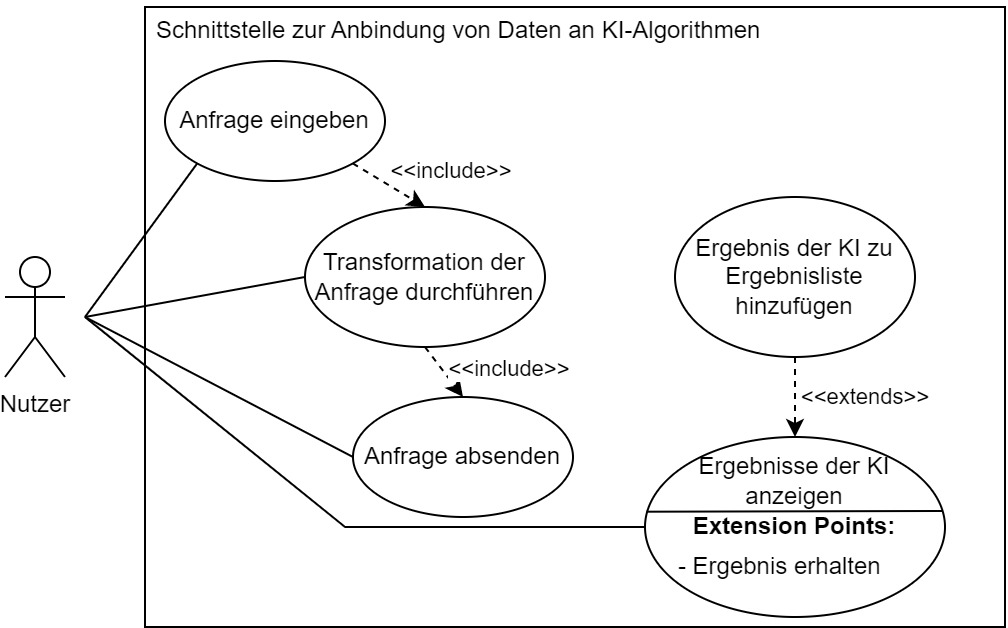
\includegraphics[width = 15cm]{bilder/UseCase}
    \caption{Use Case Diagramm der Interaktion mit der Schnittstelle}
\end{figure}

Die letzte Möglichkeit, die der Nutzer hat, mit der Schnittstelle zu interagieren, ist über die API selbst. Dort gibt es eine Route, über die die aktiven KI-Services verwaltet werden können. Abhängig von der gewählten HTTP-Methode sollen verschiedene Funktionen angeboten werden. Die drei Hauptfunktionen sind die Auflistung sämtlicher aktiven Services, das Erstellen eines neuen Services und das Löschen eines Services.

Der nächste Punkt der Anforderungsanalyse gemäß IEC 62304 ist die Festlegung des \ac{gui}. Die grafische Oberfläche sollte sich auf eine Seite beschränken und in drei Bereiche eingeteilt sein. Jeder der Bereiche beinhaltet eine Kachel mit einer Überschrift. Die drei Überschriften \glqq Query\grqq{}, \glqq Transformation\grqq{} und \glqq Service\grqq{} sollen die Aktionen innerhalb der Kachel verdeutlichen.
Der linke Bereich der Seite für die Query beinhaltet die Eingabe durch den Nutzer, welche durch ein Textfeld realisiert wird. Des Weiteren gibt es einen Button zum Hochladen der Anfrage an den Server.

Im mittleren Bereich der Seite befindet sich die Kachel für die Transformation der Eingabe. Der Inhalt der Kachel ist in drei Bereiche aufgeteilt. Der erste Bereich zeigt die vom Nutzer hochgeladene Eingabe. In diesem Feld kann der Nutzer keine Änderungen vornehmen. Das zweite Feld enthält die Eingabe für die Transformation. Das Textfeld enthält einen vorgefertigten Text in JSON-Syntax, den der Nutzer anpassen kann. Unter dem Textfeld gibt es einen Button, der die Funktion hat, die Transformationsanleitung an den Server zu senden. Das Ergebnis der Transformation wird im dritten Feld angezeigt, damit der Nutzer überprüfen kann, ob das erzeugte Ergebnis seinen Erwartungen entspricht. 

Der rechte Bereich der Seite ist für die Auswahl und Nutzung der KI-Services vorgesehen. Der gewünschte Service soll über ein Dropdown ausgewählt werden. Um den Services Anfrage-Parameter zu übergeben, wurde eine Tabellenstruktur implementiert. Die Tabelle hat zwei Spalten und beliebig viele Reihen. Innerhalb der Tabelle können Schlüssel-Wert Paare eingegeben werden, wobei der Schlüssel in der ersten Spalte und der Wert in der zweiten Spalte steht. Unter der Tabelle muss es einen Button geben, der die Anfrage an den KI-Service sendet. Daraufhin startet der Abfrageprozess der die Antworten der KI-Services zusammenträgt. Die Ergebnisse des KI-Services werden in Listenform angezeigt. Zunächst lediglich als Überschrift, erst bei einem Klick auf die Überschrift wird der Inhalt ausgeklappt.

Der nächste Punkt gemäß IEC 62304 ist die Dokumentation des Verhaltens des Systems. Besonderer Fokus liegt hierbei auf dem Verhalten gegenüber Nutzerinteraktionen. Beim ersten Besuch der Website wird dem Nutzer ein Token zugesendet, welches für die weiteren Anfragen zur Authentifizierung an der API genutzt werden soll. Innerhalb des Tokens ist eine eindeutige User-ID hinterlegt. Nachdem der Nutzer auf der linken Seite der Website in der Kachel \glqq Query\grqq{} den Upload Button gedrückt hat, sendet die Website den eingegebenen Text an die API. Dabei soll im Authorization Header der Token stehen und im Request Body der eingegebene Text in JSON-Syntax. 

Ist eine Anfrage beim Server eingegangen, wird sie in einem Redis Cache hinterlegt und anschließend an das Frontend zur Bestätigung zurückgesendet. Sollte bei der Anfrage ein Fehler aufgetreten sein, wird der Statuscode 500 an die Website zurückgegeben und das Ergebnis des Uploads wird nicht im ersten Feld der Transformation angezeigt. Ist der Upload erfolgreich, wird der Text auf der Website angezeigt. Der Nutzer hat die Möglichkeit, eine Transformationsanleitung in JSON-Syntax einzugeben und diese über den Transform-Button an das Backend zur Auswertung zu schicken. Die Transformationsanleitung wird, nachdem sie im Backend eingetroffen ist, ebenfalls im Redis Cache gespeichert. Das Backend führt eine Transformation mit der gegebenen Anleitung durch und sendet sie zurück an die Website. Das Ergebnis der Transformation wird im dritten Feld der Transformation-Kachel angezeigt. Bei einem Fehler während der Transformation wird der Statuscode 500 zurückgesendet und es werden keine Ergebnisse angezeigt.

In der Service-Kachel im rechten Bereich der Webseite kann der Nutzer über ein Dropdown einen der aktiven Services auswählen. Die Liste der Services wird beim Laden der Seite von der API angefragt. Die API führt dazu eine SQL-Anfrage in einer MySQL Datenbank aus, in der sämtliche aktiven Services hinterlegt sind. Anschließend definiert der Nutzer einen oder mehrere Parameter in einer Tabelle. Der ausgewählte Service und die eingegebenen Parameter werden durch den Klick auf einen Execute-Button unterhalb der Tabelle an die API gesendet. Das Backend soll die transformierten Anfragen über RabbitMQ an den dafür vorgesehenen Service schicken. Zur Bestimmung des Services wird der von der API mitgesendete Service-Name genutzt, der durch die Dropdown-Auswahl ermittelt wird. Jede einzelne Anfrage hat eine Anzahl an erwarteten Antworten. Das Backend sendet die Gesamtzahl der erwarteten Antworten an die Website. Dort wird die Antwortzahl für eine Fortschrittsanzeige verwendet werden.

Der zu implementierende Service beinhaltet eine Textähnlichkeitssuche. Dieser Service erhält die vom Backend gesendeten Anfragen. Mittels des BERT-Modells werden die semantisch ähnlichsten Texte aus einer Elasticsearch-Datenbank herausgefiltert. RabbitMQ sendet die ähnlichsten Texte im Anschluss an das Backend. Dort werden sie im Redis-Cache zwischengespeichert. Die Website soll nach dem Absenden der Anfrage durch den Nutzer in regelmäßigen Intervallen selbständig Anfragen an die API stellen, ob Antworten vom KI-Service im Backend eingetroffen sind. Bei einer solchen Anfrage überprüft das Backend im Redis-Cache, ob eine oder mehrere Antworten eingetroffen sind und sendet diese an die Website. Liegen noch keine Antworten im Redis-Cache, sendet die API die Nachricht \texttt{successful:False}. Die Website stellt so lange Anfragen an die API, bis die erwartete Zahl der Antworten eingetroffen ist.

Der nächste Punkt in der IEC 62304 ist die Festlegung der Geschwindigkeit, in der das System bestimmte Aufgaben abarbeiten soll. Hierzu gab es bezüglich der KI-Services keine genaue Vorgabe seitens CONET. Das Backend und die Kommunikation zu den einzelnen Services hatte jedoch gewisse Maximallaufzeiten. Eine Anfrage, die durch einen HTTP-Request in der API ankommt, soll maximal 0,5 Sekunden benötigen, um an den richtigen Service weitergeleitet zu werden. Die Rückrichtung vom Service zum Backend soll ebenfalls maximal 0,5 in Anspruch nehmen. Die Gesamtzeit der Kommunikation zwischen Backend und einem Service darf demnach nicht mehr als eine Sekunde betragen. Da der KI-Algorithmus keine festgelegte Laufzeit hat, soll durch die Architektur, mit der die Systeme aufgesetzt sind, kein großer zusätzlicher Overhead entstehen. Antwortzeiten innerhalb einer Sekunde gelten laut CONET als responsiv und praxistauglich.

In der Spezifikation IEC 62304 wird ebenfalls gefordert, die Umgebung, in der die Software installiert werden soll, zu definieren. Die Hauptanforderung CONET war hierbei, dass das System möglichst plattformunabhängig entwickelt werden soll. Für die Installation der einzelnen Komponenten ist Docker vorgesehen.

Der letzte für die Anforderungsanalyse relevante Punkt aus der IEC 62304 ist die Beschreibung, wie das System auf Benutzerfehler und Überlast reagieren soll. Grundsätzlich sollen Benutzerfehler im Backend abgefangen werden und nicht zum Serverabsturz führen. Dazu soll ein System implementiert werden, das potentielle Fehler abfängt und anschließend in eine MySQL-Datenbank logged. Des Weiteren sollen die aufgerufenen Routen und Vorgänge innerhalb des Backends sowie den einzelnen Services geloggt werden. Dadurch kann nachvollzogen werden, ob das System ordnungsgemäß funktioniert. Die Architektur soll horizontal skalierbar sein, wodurch mehrere Instanzen der API und der einzelnen Services parallel betrieben werden können. Jede dieser Instanzen muss für sich allein voll funktionsfähig sein.

\subsection{Konzeption}
\subsubsection{Softwarearchitektur}
Ein grundlegender Dienst, der Daten mit einer KI verbindet, kann mithilfe eines einzigen Python-Scripts erstellt werden. Die Herausforderung an einer praxistauglichen Anwendung, die gleichzeitig von mehreren Usern genutzt werden kann, liegt im  Architekturdesign der Software. Eine praxistaugliche Anwendung muss neben den funktionalen Anforderungen auch noch weitere nicht funktionale Anforderungen erfüllen. Laut CONET sind die drei wichtigsten nicht funktionalen Anforderungen Performance, Skalierbarkeit und Verfügbarkeit. Die drei Anforderungen können mit einem lokal ausgeführten Skript nicht erfüllt werden. 

Damit Nutzer mit der Software interagieren können, wird ein Frontend benötigt. Ein zentral gehostetes, webbasiertes Frontend kann von einem Nutzer über eine einfache URL im Webbrowser aufgerufen werden. Für die anzuzeigenden Daten im Frontend wird eine Verbindung zum Backend benötigt. Diese wird über eine HTTP Verbindung zur mit Flask gehosteten REST API bereitgestellt.

Um die Anforderung der Skalierbarkeit erfüllen zu können, ist die REST-API komplett zustandslos implementiert worden. Eine API ohne Zustände speichert keine Zwischenstände zu den Anfragen einzelner Nutzer. Bei jeder Anfrage an die API müssen sämtliche Informationen im Request bereitgestellt werden, die die API zum Bearbeiten der Anfrage benötigt. Dies bietet die Möglichkeit bei steigender Nutzerzahl mehrere parallel betriebene Instanzen der API hochzufahren. Dadurch ist eine horizontale Skalierung gewährleistet. Horizontal skalierbare Instanzen innerhalb der Softwarearchitektur sind in Abbildung 6 mit zwei hintereinander gestapelten Rechtecken visualisiert.

Da die Kommunikation zwischen dem Frontend, der API und den KI-Services asynchron läuft, muss das Flask-Backend trotz seiner Zustandslosigkeit Transformationsanleitungen und Ergebnisse der KI-Services zwischenspeichern, bis sie im Frontend benötigt werden. Um die Performanceanforderungen erfüllen zu können, können nicht sämtliche Zwischenstände in einer MySQL-Datenbank gespeichert werden. Die Lese- und Schreibgeschwindigkeit kann bei steigender Nutzerzahl problematisch werden. Um dem Entgegenzuwirken, wird mit Redis ein Key-Value-Store als Cache betrieben. Die zwischengespeicherten Daten werden nach dem ersten Aufruf wieder gelöscht, weswegen eine persistente Speicherung nicht notwendig ist. In-Memory Datenbanken speichern und führen ihre Queries direkt im RAM aus, wodurch Anfragen im Vergleich zu einer MySQL-Datenbank deutlich schneller ausgeführt werden.

Im Flask-Backend werden sämtliche Routen und die meisten Funktionen abgekapselt in einem Funktion Wrapper ausgeführt. Dieser fungiert als eine Art Sandbox, in der auftretende Fehler nicht zum Programmabsturz führen, sondern behandelt und geloggt werden können. Die Logs werden persistent in einer MySQL-Datenbank gespeichert. Mit dem Dienst Grafana können diese Logs angezeigt werden.

Die Laufzeit von KI-Services kann sehr stark vom verwendeten KI-Modell, der zu durchsuchenden Datenmenge, wie auch der vom Nutzer gesendeten Eingabe abhängen. Bei einer synchronen Kommunikation zwischen dem Flask-Backend und dem Service können sehr lange Wartezeiten entstehen. Wenn der KI-Service ebenfalls eine REST-Schnittstelle implementieren würde, könnten es bei einem HTTP-Request zum Timeout der Anfrage führen. Aufgrund der schwanken Laufzeit muss eine asynchrone Kommunikationsstruktur, wie RabbitMQ mit dem AMQP implementiert werden.

Die einzelnen Services können mit einem Eintrag in der MySQL-Datenbank registriert werden. Für die Registrierung muss lediglich der Name und der im Frontend anzuzeigende Name des Services hinterlegt werden. Die Registrierung eines Dienstes kann durch den Aufruf einer Route in der API durchgeführt werden. 

Der im Prototyp implementierte KI-Service nutzt das BERT-Modell von Google zum Konvertieren der Nutzereingaben in semantische Vektoren. Es wird ebenfalls eine Elasticsearch-Datenbank betrieben, in der die zu durchsuchenden Einträge gespeichert sind. Im Gegensatz zu einer MySQL-Datenbank, kann in einer Elasticsearch-Datenbank zu jedem Eintrag ein semantischer Vektor gespeichert werden. Der KI-Service kann mithilfe der Kosinusähnlichkeitssuche den semantischen Vektor der Eingabe mit den Vektoren der Datenbank vergleichen und so die semantisch ähnlichsten Texte herausfiltern. Die gefunden Einträge werden über RabbitMQ im Anschluss wieder an das Flask-Backend geschickt, damit sie dort vom Frontend ausgelesen werden können.

\begin{figure}[H]
  \centering
    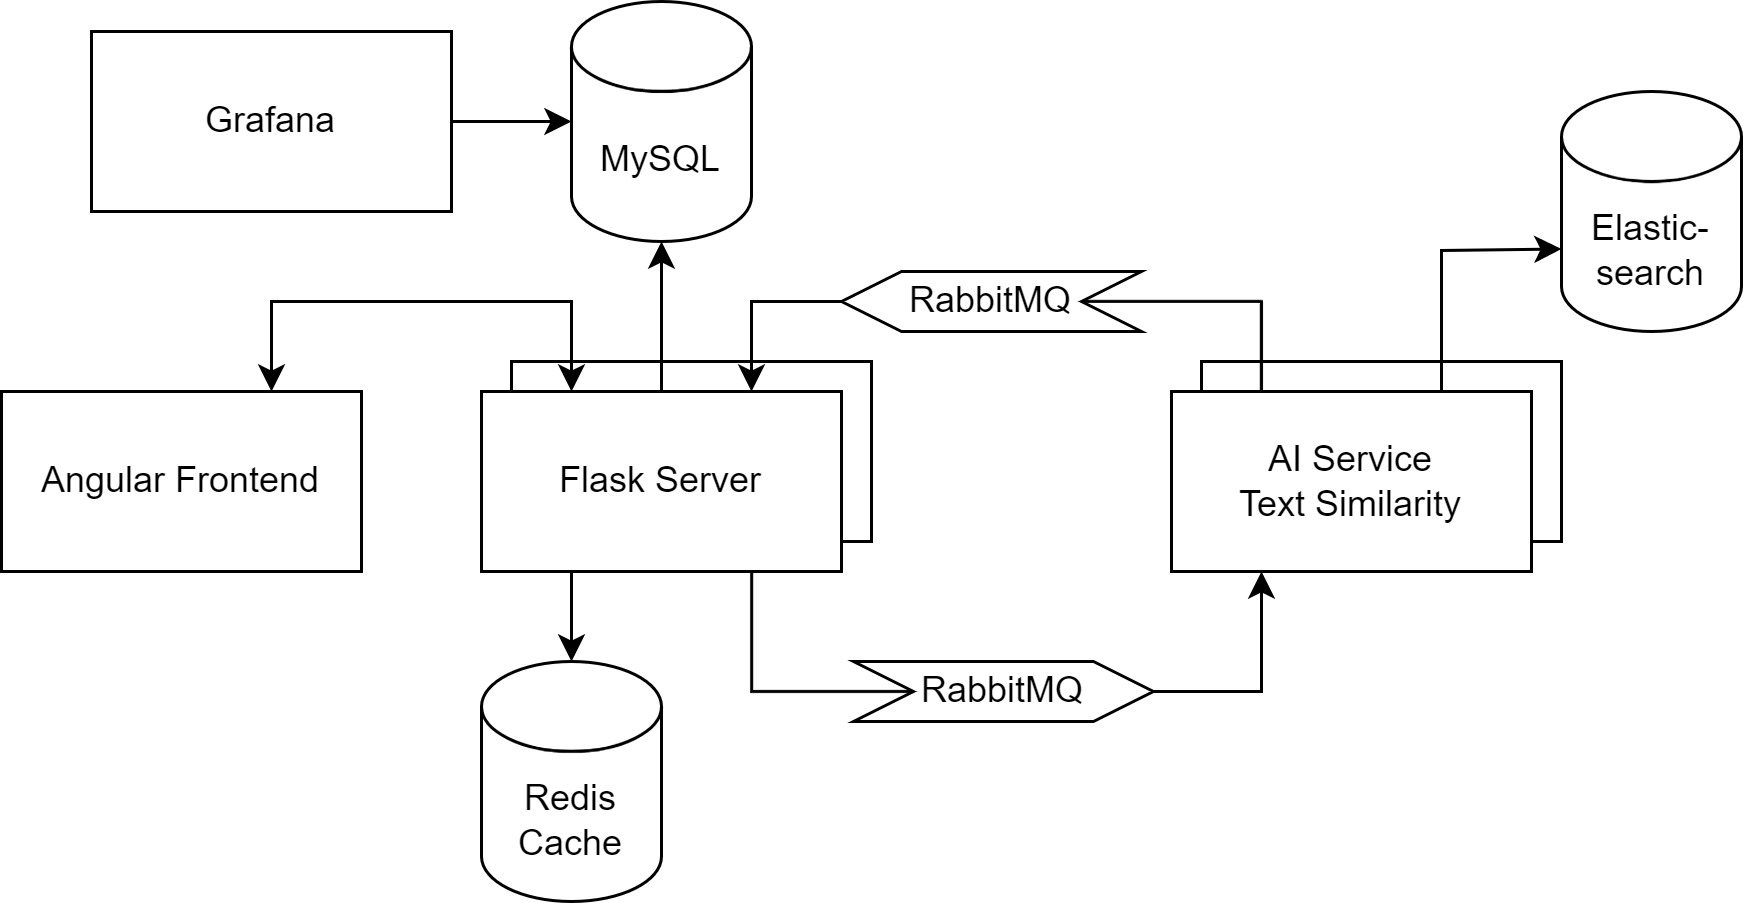
\includegraphics[width = 12cm]{bilder/Architektur}
    \caption{Softwarearchitekturdiagramm}
\end{figure}

\subsubsection{Programmablauf}
\begin{figure}[H]
  \centering
    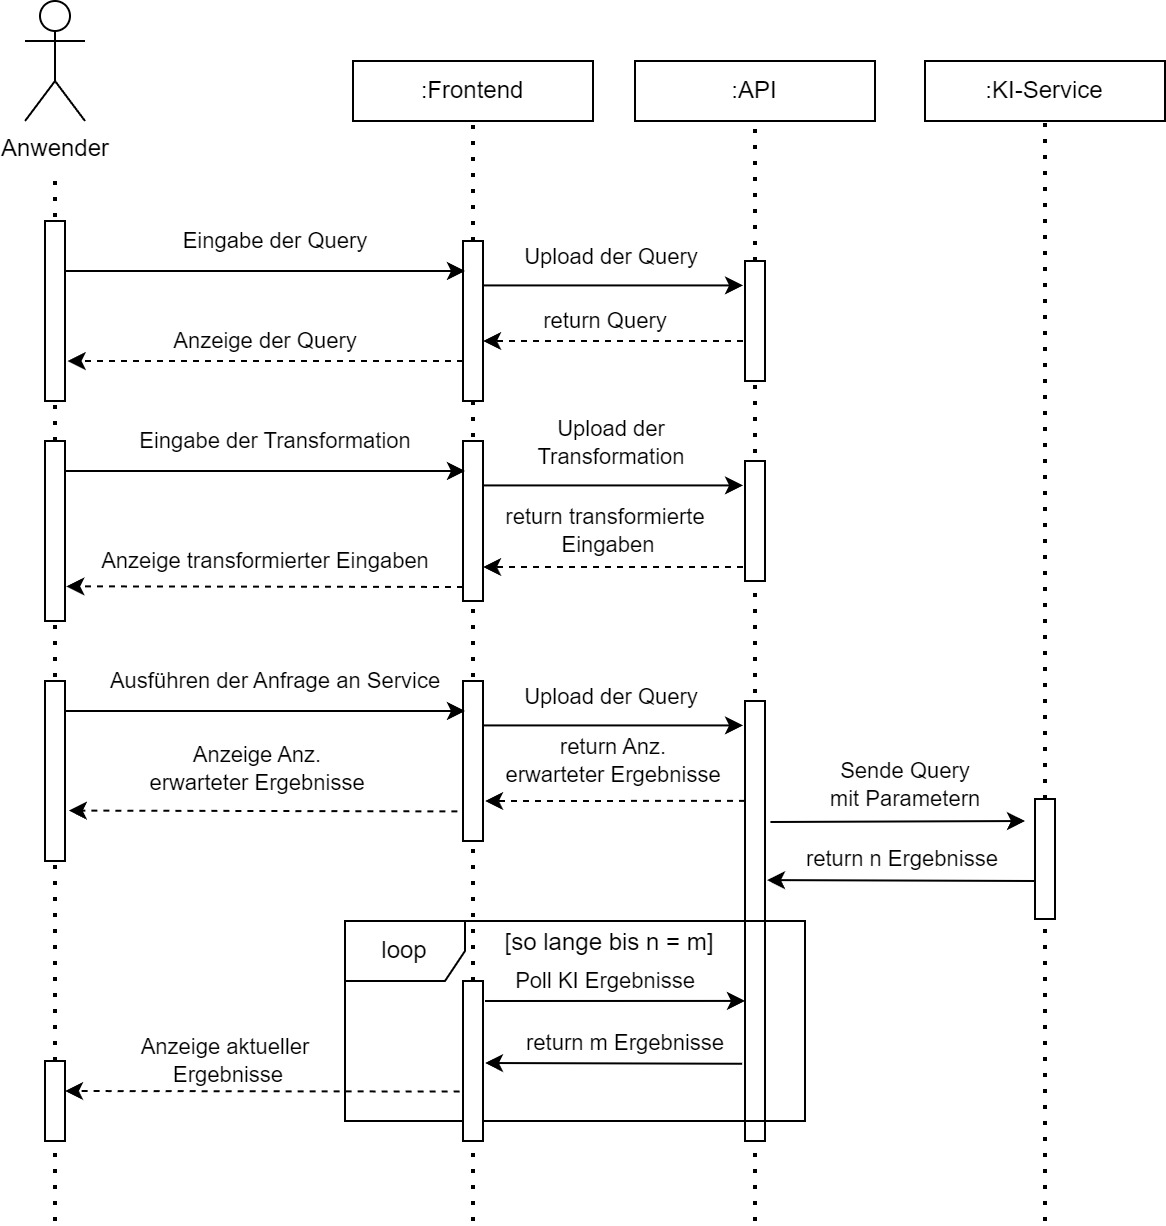
\includegraphics[width = 15cm]{bilder/ArchitekturSequenz}
    \caption{UML-Sequenzdiagramm des Programmablaufs}
\end{figure}

Das Ziel der Bachelorarbeit ist es, eine Schnittstelle zu entwickeln, die Daten an KI-Algorithmen anbindet. Dazu wird im Prototyp ein System implementiert, welches die Anbindung in drei Schritten durchführt. In Abbildung 7 ist der grundlegende Programmablauf in einem UML-Sequenzdiagramm dargestellt. In Abbildung 8 ist ein Mockup der gesamten Website abgebildet. Die Interaktionen, die der Anwender auf der Website tätigen kann, sind hier beispielhaft abgebildet. Die Mockups dienen der Veranschaulichung des entwickelten Konzepts für die Nutzerinteraktion mit der Schnittstelle. 

\begin{figure}[H]
  \centering
    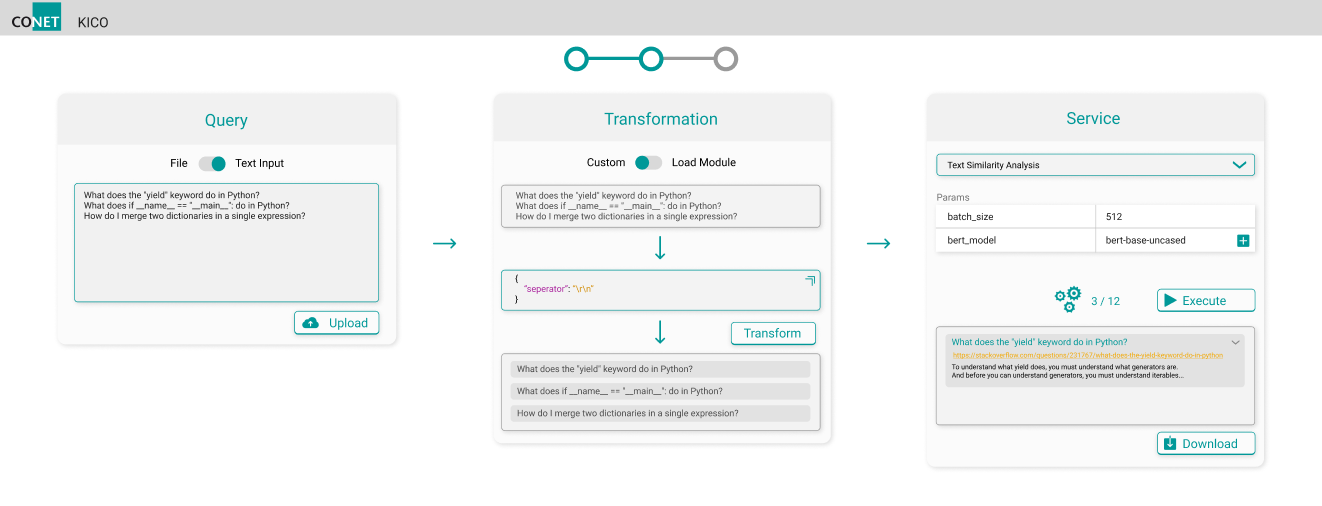
\includegraphics[width = 15cm]{bilder/mockup}
    \caption{Mockup Frontend}
\end{figure}

Der erste Schritt ist, wie auch in den Anforderungen definiert, die Eingabe der Query durch den Anwender. Auf der Website gibt es dafür ein Textfeld, in dem diese Eingabe stattfindet. Eine Darstellung der \glqq Query\grqq{} Kachel ist in Abbildung 9 gegeben. Die Eingabe kann durch einen Klick auf den \glqq Upload\grqq{} Button an die API per HTTP-POST-Request geschickt werden. Innerhalb des Bodys befindet sich die Eingabe. Zusätzlich zu dem Body wird ein Authorization Header mitgeschickt, der die User-ID des Anwenders enthält. Innerhalb der API wird die User-ID als Schlüssel und die Query als Wert für einen Eintrag in den Redis-Cache genutzt. Die Eingabe wird im Backend zunächst nur zwischengespeichert. Als Bestätigung für den Nutzer, sendet die API die erhaltene Query wieder an die Website zurück. Dort wird sie im oberen Bereich der \glqq Transformation\grqq Kachel angezeigt. 

\begin{figure}[H]
  \centering
    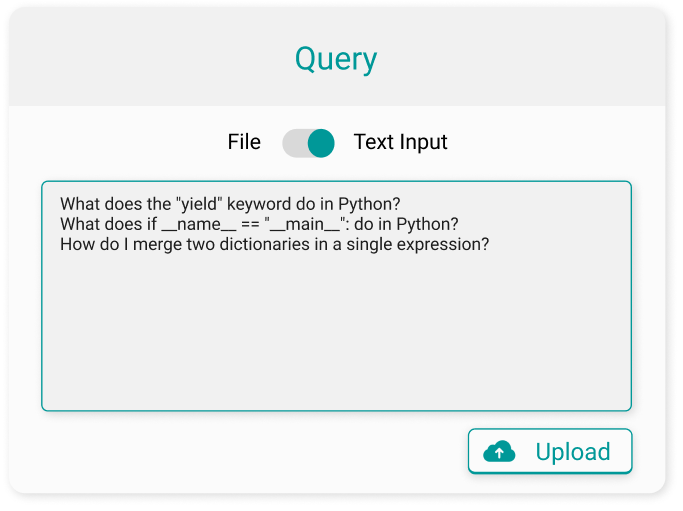
\includegraphics[width = 10cm]{bilder/mockupQuery}
    \caption{Mockup Query}
\end{figure}

Der zweite Schritt ist die Eingabe der Transformationsanleitung. In Abbildung 10 ist das Mockup für die Transformation-Kachel abgebildet. Im mittleren Textfeld der Transformation-Kachel ist für diesen Schritt ein Textfeld vorgesehen. Nach Abschluss der Eingabe kann der Anwender auf den Transform-Button klicken, um die Eingabe an die API hochzuladen. Wie auch bei dem Upload der Query wird die User-ID im Header des Requests mitgeschickt. Die API nutzt die User-ID um die zuvor hochgeladene Query aus dem Redis-Cache zu laden. Die im Request mitgelieferte Transformationsanleitung wird in diesem Schritt genutzt, um die Query zu transformieren. Im Prototyp wird eine Split-Operation beliebige Anzahl an Replace-Operationen implementiert. Die Split-Operation teilt die Query in mehrere einzelne Queries. Dazu wird eine Zeichenkette genutzt, die als Trennzeichen dient. Die Replace-Operation ersetzt eine eingegebene Zeichenkette durch eine andere. Das Ergebnis der Transformation wird innerhalb der Response wieder an die Website gesendet. Sollte eine Split-Operation angegeben worden sein, werden die daraus resultierenden Queries im unteren Bereich der Transformation-Kachel angezeigt. 

\begin{figure}[H]
  \centering
    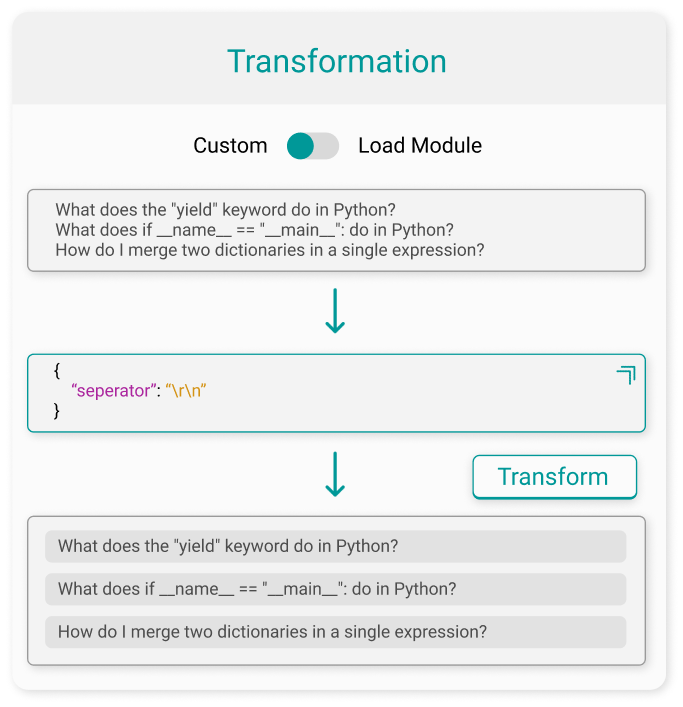
\includegraphics[width = 10cm]{bilder/mockupTransformation}
    \caption{Mockup Transformation}
\end{figure}

Der dritte Schritt ist die Ausführung der Anfrage durch einen KI-Service. In Abbildung 11 ist das Mockup für die Service-Kachel dargestellt. Der Anwender  wählt im Dropdown der Serivce-Kachel einen der in der MySQL Datenbank hinterlegten aktiven Services aus und gibt anschließend einen oder mehrere Parameter in die Tabelle unterhalb des Dropdowns ein. Durch einen Klick auf den Execute-Button wird eine Query im Frontend zusammengebaut und als Request an die API gesendet. Innerhalb der Query befindet sich der Name des KI-Services, sowie die in der Tabelle definierten Parameter. Wenn der Request bei der API eingegangen ist, lädt das Backend sowohl die in Schritt eins eingegebene Query, sowie die in Schritt zwei eingegebene Transformationsanleitung. Das Backend führt nun eine erneute Transformation durch und sendet dem Frontend die Anzahl der erwarteten Antworten des KI-Services zurück. Die Anzahl setzt sich aus der Menge der durch die Split-Operation entstandenen Queries und den eingegebenen Parametern zusammen. Für den KI-Service zur Textähnlichkeitssuche gibt es den Parameter \texttt{search\_{}size}. Die Anzahl der erwarteten Antworten wird im Frontend zunächst zur Fortschrittsanzeige genutzt. Der zweite Einsatzzweck der erwarteten Antworten ist innerhalb der darauffolgenden Schleife. Nach dem Upload der Query startet die Website eine Schleife in der bei der API regelmäßig nach neuen Ergebnissen des KI-Services gefragt wird. Der KI-Service bekommt direkt nach dem Upload der Query über RabbitMQ die Anfrage zugesendet. Innerhalb des Services in dem die Textähnlichkeitssuche  implementiert wird, wird die eingehende Nachricht angenommen und mithilfe des BERT-Modells in einer Elasticsearch Datenbank nach den semantisch ähnlichsten Einträgen gesucht. Es werden, abhängig von der \texttt{search\_{}size}, die ähnlichsten Ergebnisse gesammelt und über RabbitMQ wieder an das Backend gesendet. Im Sequenzdiagramm in Abbildung 7 ist die Anzahl mit der Variable \texttt{n} angegeben. Die Ergebnisse werden in einem Redis-Cache zwischengespeichert. Wie zuvor erwähnt, läuft parallel zu der Bearbeitung der Services im Frontend eine Schleife, die die Ergebnisse aus der API abfragt. In einer Schleifeniteration werden sämtliche im Redis-Cache hinterlegten Ergebnisse aus dem KI-Service abgefragt und an das Frontend gesendet. Die maximale Anzahl der Ergebnisse ist dabei \texttt{m}. Die Schleife läuft so lange, bis die Anzahl der erhaltenen Antworten identisch mit Anzahl der erwarteten Antworten ist, also bis $n=m$ ist. Jedes erhaltene Ergebnis wird im Frontend im unteren Bereich der Service-Kachel angezeigt. Damit ist der Programmablauf abgeschlossen und der Anwender kann eine neue Query eingeben.

\begin{figure}[H]
  \centering
    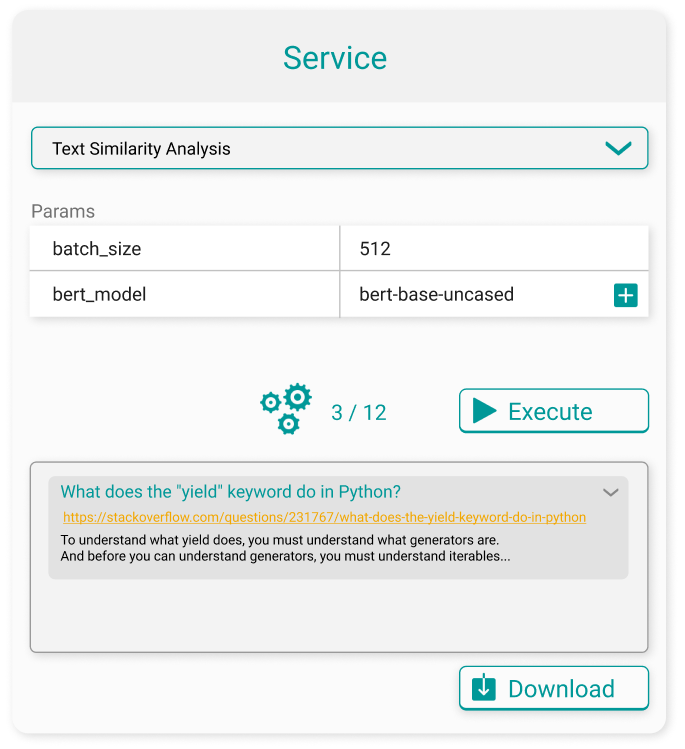
\includegraphics[width = 7.5cm]{bilder/mockupService}
    \caption{Mockup Service}
\end{figure}

\subsection{Prototypische Umsetzung}
\subsubsection{Implementierung der REST-API}
Python bietet mit dem Package Flask die Möglichkeit einen simplen und gut skalierbaren Webserver aufzusetzen. Für das Starten einer Flask-Instanz muss das Package Flask in die Python Umgebung importiert werden. Anschließend kann ein Flask-Objekt erzeugt und die Flask-Instanz mit den gewünschten Parametern gestartet werden.

\begin{lstlisting}[language=Python, caption={Aufsetzen einer Flask-Instanz}]
from flask import Flask
app = Flask(__name__)
app.run(host="0.0.0.0", port=80, use_reloader=False)
\end{lstlisting}

Damit die API auch automatisiert aus einem Docker-Container heraus gestartet werden kann, muss die Ausführung des Flask-Services in die Main Methode von Python ausgelagert werden. Flask blockiert den Thread, auf dem es ausgeführt wird, was eine asynchrone Kommunikation über RabbitMQ nicht möglich macht. Der Receiver benötigt seinen eigenen Thread, weswegen eine Multithreading-Architektur implementiert werden muss. Zu diesem Zweck wird das \texttt{threading} Package genutzt. Über den Parameter \texttt{daemon} kann bei der Erzeugung eines Threads festgelegt werden, dass der Thread im Hintergrund läuft und den Haupt-Thread nicht blockiert.

\begin{lstlisting}[language=Python, caption={Flask im eigenen Thread starten}]
def start_server():
    app.run(host="0.0.0.0", port=80, use_reloader=False)

if __name__ == '__main__':
    thread_server = threading.Thread(target=start_server, daemon=True).start()
\end{lstlisting}

Eine in der API adressierbare Route kann in Flask über Function-Annotations definiert werden. Die von Flask implementierten Anntotations haben die Form \texttt{instanz.route('path', methods=["METHOD"])}. Der Name der Instanz wird am Anfang des Projekts als \texttt{app} definiert. Der \texttt{path} beschreibt die Route, die vom Frontend aufgerufen werden muss, damit die nachfolgende Funktion ausgeführt wird. Im Array \texttt{methods} besteht die Möglichkeit, ein oder mehrere Request-Typen zu definieren, die die Funktion akzeptieren soll.

Eine beispielhafte Nutzung der Annotations, um eine Route in der API zu definieren, ist nachfolgend aufgeführt. 

\begin{lstlisting}[language=Python, caption={Beispiel einer API-Routendefinition über Annotations}]
@app.route('/', methods=["GET"])
def index():
    [..]
    return r.respond({"token": token}, cookie=f"Authorization={token}")
\end{lstlisting}

Der Inhalt der Methode und deren genaue Funktionsweise wird in den folgenden Kapiteln näher erläutert.

Die Funktion \texttt{respond} ist im Skript \texttt{api/response\_{}generator.py} definiert. Sie dient als Function-Wrapper, der bei jeder ausgehenden Response die Response-Header, eventuelle Cookies und den Reponse-Typen setzt. Der Output der Response wird mithilfe des \texttt{json} Packages in JSON-Syntax konvertiert.

\begin{lstlisting}[language=Python, caption={Respond Funktion zur Rückgabe von JSON-Responses}]
import json
from flask import Response
def respond(r, status=200, json_dump=True, cookie=""):
    [...]
    return Response(json.dumps(r), status=status, mimetype='application/json', headers=headers)
\end{lstlisting}

In Tabelle 1 sind die in der API verfügbaren Routen aufgelistet. Auf die genaue Funktionalität der einzelnen Funktionen wird in den folgenden Kapiteln eingegangen.

\begin{table}[H]
\centering
\begin{tabular}{c|c|l}
\textbf{Route} & \textbf{Typ} & \textbf{Funktion}\\
\hline
\texttt{'/'} & \texttt{GET} & Erstellung eines JSON-Web-Tokens\\
\hline
\texttt{'/upload/file'}  & \texttt{POST} & Hochladen einer Textdatei für den Input der KI \\
\texttt{'/upload/text'}  & \texttt{POST} & Texteingabe für den Input des KI-Services \\    
\texttt{'/transform'}  & \texttt{POST} & Festlegen der Tranformationseigenschaften\\ 
\texttt{'/send'}  & \texttt{POST} & Transformieren und Senden des Inputs an einen KI-Service \\ 
\texttt{'/poll'}  & \texttt{GET} & Abfrage der vom KI-Service gelieferten Ergebnisse \\ 
\hline
\texttt{'/service'}  & \texttt{GET} & Auflistung der Services \\
\texttt{'/service'}  & \texttt{POST} & Registrieren eines neuen Services \\ 
\texttt{'/service'}  & \texttt{DELETE} & Löschen eines Services \\       
\end{tabular}
\caption{Implementierte Routen der REST-API}
\end{table}

\subsubsection{Nutzeridentifizierung mit JWT}
Innerhalb des Backendes ist es notwendig, einzelne Nutzer voneinander zu unterscheiden. Für jeden Nutzer speichert das Backend den hochgeladenen Text, die Transformationsanleitung und die Antworten des angefragten KI-Services im Redis-Cache. Um Nutzer voneinander unterscheiden zu können, gibt es zwei grundlegende Möglichkeiten. 
\begin{enumerate}
\item Identifizierung durch den Nutzer der Software. Beispielsweise mittels Registrierung durch E-Mail Adresse und Passwort.
\item Identifizierung durch das Backend der Software. Generierung und Zuweisung einer zufälligen, aber eindeutigen User-ID.
\end{enumerate}

Die Erhebung von personenbezogenen Daten setzt die Einhaltung der \ac{dsgvo} voraus. Dies bedeutet einen erheblichen Mehraufwand für eine Anwendung, die sonst keinen weiteren Nutzen aus den Daten zieht.

Das Backend nutzt einen \ac{uuid} der sich durch das Python Package \texttt{uuid} generieren lässt. Eine UUID ist eine 32 Zeichen lange Zahl im Hexadezimalformat. Die importierte Funktion \texttt{uuid4()} erzeugt eine zufällige, ohne von Parametern beeinflusste UUID. Der Nutzer muss diese UUID mitgeteilt bekommen und für seine Anfragen, aufgrund der zustandslosen Implementierung der API, im Authorization Header mitschicken. Damit die UUID nicht ausgelesen oder manipuliert werden kann, wird sie nicht als einfacher Text in der Response an den Nutzer geschickt, sondern vorher in ein JSON Token geschrieben und verschlüsselt.

Ein \ac{jwt} ist ein kompaktes, URL-sicheres Mittel zur Darstellung von Forderungen, die zwischen zwei Parteien übertragen werden sollen. Die Angaben in einem JWT werden als JSON-Objekt kodiert. Der Inhalt des JWT kann digital signiert oder die Integrität mit einem \ac{mac} geschützt und/oder verschlüsselt werden.\footcite{jones2015json}

Im nachfolgenden Codeausschnitt ist die Generierung der UUID und die Verschlüsselung des JWT dargestellt.
\begin{lstlisting}[language=Python, caption={Generierung der UUID und Erstellung des JWT}]
def uuid_gen():
    return uuid.uuid4()
    
def encode_token(param):
    return jwt.encode(param, JWT_PASSWORD, algorithm="HS256")

token = encode_token({'uid': str(uuid_gen())})
\end{lstlisting}

Für jede Route, ausgenommen die \texttt{/service} Routen zum Management der Services, wird der JWT für die Ausführung benötigt. Die Überprüfung und Entschlüsselung des Tokens ist für jede Route gleich, daher ist es sinnvoll diese Funktionalität zu zentralisieren. Damit wird die Fehleranfälligkeit reduziert und und die Wartbarkeit erhöht, sollte sich zum Beispiel der Algorithmus oder das Passwort für die Verschlüsselung ändern. Wie auch Flask-Annotations zum Definieren einer Route verwendet, ist es möglich eigene Annotations zu entwerfen. Für diese Funktion ist das Python Package \texttt{functools} mit der Funktion \texttt{wraps} zuständig. Wraps ermöglicht es, Funktionen ineinander zu verschachteln.

Im Prototyp wird die Funktion \texttt{token\_{}required(f)} definiert. Diese Funktion dient als eine Umgebung, in der eine weitere Funktion ausgeführt werden. Im Gegensatz zur normalen Ausführung einer Funktion, werden in der \texttt{token\_{}required(f)} Funktion vor der Ausführung der eigentlichen Funktion mehrere Rahmenbedingungen geprüft. Der vom Nutzer gesendete Token muss nach erfolgreicher Entschlüsselung syntaktisch korrektes JSON enthalten. Sollte dies nicht der Fall sein, wird die die eigentliche Funktion, die zur API Route gehört, gar nicht erst ausgeführt. Der Nutzer bekommt direkt eine Response mit dem HTTP-Error-Code 401: Unauthorized gesendet. \footcite{fielding1999rfc2616}

Wenn die Entschlüsselung des Tokens erfolgreich war, wird die innere Funktion ausgeführt. Als Parameter der inneren Funktion wird die im JWT enthaltene UUID übergeben. Durch diesen Aufbau ist der Code für die Verifizierung des Tokens und die Logik der Funktion unter der angesprochenen Route vollständig getrennt.

\begin{lstlisting}[language=Python, caption={Route zum Upload von Queries mit Nutzung des JWTs}]
@routes.route('/upload/text', methods=['POST'])
@token_required
def upload_text(uid):
    [...]
\end{lstlisting}

\subsubsection{Caching mit Redis Datenbank}
Redis ist ein Key-Value-Store der vollständig im RAM ausgeführt wird. Innerhalb von Redis sind mehrere Datenbanken definiert, die in ihrer Standartkonfiguration über einen Index $i$, mit $0\leq{}i<16$ aufgerufen werden. Im Backend werden die ersten drei Datenbanken verwendet.
\begin{enumerate}
 \item Datenbank 0: Cache der hochgeladenen Queries für den Input der KI
 \item Datenbank 1: Cache der Transformationsanleitung
 \item Datenbank 2: Cache der vom KI-Service produzierten Ergebnisse
\end{enumerate} 

Redis wird zum Cachen von Nutzereingaben und für die Zwischenspeicherung von Ergebnissen aus den KI-Services verwendet. In der ersten Datenbank werden die vom Nutzer eingegebenen Queries gespeichert. Redis kann grundsätzlich nur textbasierte Daten speichern. Dies reicht für den Anwendungsfall der Software jedoch aus. Um die Query in Redis speichern zu können, muss zunächst eine Verbindung zum Redis Cache aufgebaut werden. Die URL, unter der Redis erreichbar ist, wird aus den Environmentvariablen bezogen. Im ersten Schritt wird ein \texttt{ConnectionPool} angelegt. Dieser verbindet sich unter einem angegebenen Host, einem Port mit einer Datenbank. Anschließend kann im zweiten Schritt eine Redis-Instanz in Python erstellt werden. Diese bekommt den \texttt{ConnectionPool} als Argument übergeben. Innerhalb der Redis-Instanz befinden sich die benötigten Funktionen, um mit der Redis-Datenbank arbeiten zu können.

\begin{lstlisting}[language=Python, caption={Aufsetzen der Redis-Verbindung}]
redis_host = os.environ.get('REDIS_HOST')
pool_upload = redis.ConnectionPool(host=redis_host, port=6379, db=0)
red_upload = redis.Redis(connection_pool=pool_upload)
\end{lstlisting}

In der Redis-Instanz werden zwei Funktionen definiert, die im Prototyp Verwendung finden. Die \texttt{set(k,v)} Methode nimmt einen Schlüssel als ersten Parameter und einen Wert als zweiten Parameter an. Das übergebene Key-Value-Paar wird mit diesem Methodenaufruf entweder neu in der Datenbank angelegt oder falls bereits ein identischer Schlüssel vorhanden sein sollte, mit den aktuellen Werten überschrieben. Das Zwischenspeichern der hochgeladenen Query ist im nachfolgenden Codeausschnitt abgebildet.  

\begin{lstlisting}[language=Python, caption={Set-Funktion aus Redis}]
red_upload.set(uid, body['text'])
\end{lstlisting}

Die zweite Funktion der Redis-Instanz ist die \texttt{get(k)} Methode. Diese bekommt einen Schlüssel übergeben und gibt den dazugehörigen Wert zurück. Das nachfolgende Codesegment stammt aus der Transform-Route. Hier wird die zwischengespeicherte Query, sowie die Transformationsanleitung aus dem Redis Cache geladen. Wichtig dabei zu beachten ist es, dass die aus dem Redis-Cache geladenen Werte noch in ein Zeichenformat konvertiert werden müssen. In diesem Fall ist die Kodierung UTF-8 gewählt worden, da diese die meisten Sonderzeichen unterstützt.

\begin{lstlisting}[language=Python, caption={Get-Funktion aus Redis}]
messages = transform(red_upload.get(uid).decode('utf-8'), red_transform.get(uid))
\end{lstlisting}

\subsubsection{Kommunikation zwischen Backend und Services mit RabbitMQ}
Für den Informationsaustausch zwischen dem Backend und den verschiedenen KI-Services ist eine asynchrone Kommunikation implementiert. Je nach Komplexität des Services, kann die Verarbeitung einer vom Nutzer gestellten Anfrage mehrere Sekunden bis Minuten dauern. Eine synchrone Kommunikation, in der der Client auf unbestimmte Zeit auf eine Antwort wartet, ist nicht möglich. Wenn nach einer vom Browser definierten Zeit keine Antwort auf den Request kommt, wird der Request mit einem Timeout abgebrochen. Sollte die KI nach der maximal verfügbaren Zeit ihr Ergebnis liefern, wird dieses Verworfen und der Nutzer muss eine neue Anfrage stellen. Damit Anfragen nicht verloren gehen und die Antworten dem Server mitgeteilt werden können, wenn sie bereit sind, wird der Message Broker RabbitMQ implementiert. 

RabbitMQ dient als Middleware, die Anfragen vom Server annimmt und diese im in einer Queue zwischenspeichert, um sie anschließend an die Services zu verteilen. Damit die Nachrichten in eine Queue geschrieben werden können, muss im ersten Schritt eine Verbindung zu RabbitMQ aufgebaut werden. Mithilfe des Packages \texttt{pika} kann über den Host, unter dem RabbitMQ erreichbar ist, den Port 5672 und den Login-Credentials eine TCP Verbindung aufgebaut werden.

Innerhalb einer Connection, können über einen Channel können sowohl der Server als auch die Services eine Verbindung mit dem RabbitMQ Dienst aufbauen. Ein Channel beschreibt die logische Verbindung zwischen dem Server/Service und dem Broker. Für jede TCP Verbindung mit RabbitMQ können mehrere Channels erstellt werden.\footcite{dossot2014rabbitmq}

In einem Channel wird letztendlich die Queue definiert, in der die Nachrichten zwischengespeichert werden. Im folgenden Codeausschnitt ist gezeigt, wie eine Connection, ein Channel und eine Queue erstellt werden.

\begin{lstlisting}[language=Python, caption={Verbindung zu RabbitMQ und Erstellung eines Channels und einer Queue}]
def produce(uid, service, query, params):
    connection = pika.BlockingConnection(pika.ConnectionParameters(rabbit_host, 5672, '/', credentials))
    channel = connection.channel()
    channel.queue_declare(queue=service)
\end{lstlisting}

Die Nachrichten, die der Server an die Services schickt, werden mittels der im Channel definierten Methode \texttt{basic\_{}publish} in die für den Service entsprechende Queue geschrieben werden. Im vorherigen Codeausschnitt wird der Parameter \texttt{service} in der \texttt{produce} Methode übergeben. Dieser ist abhängig vom Service, an den die Anfrage gerichtet ist. Im Prototyp wurde der Service \texttt{text-similarity} implementiert. Dieser kann im Frontend als Ziel ausgewählt werden. Wenn der Nutzer im Frontend die Anfrage an den \texttt{text-similarity} Service stellt, wird die Methode \texttt{produce} mit dem String \texttt{\glqq text-similarity\grqq{}} aufgerufen.

Sollte es die Queue mit dem aufgerufenen Service noch nicht geben, wird diese von RabbitMQ beim ersten Aufrufen erstellt. Ist sie bereits vorhanden, wird lediglich ein Eintrag in die entsprechende Queue geschrieben.

Die Nachricht, welche aus der Anfrage des Nutzers, den eingegebenen Parametern und weiteren im Backend automatisch generierten Parametern, wie dem UUID, besteht, wird anschließend mittels AMQP an den Rabbit Broker gesendet. Dort wird die Nachricht, wie zuvor beschrieben, in die entsprechende Queue eingetragen. 

Auf Seiten des Services wird eine Methode implementiert, die die Nachrichten in einer Queue auslesen kann. Zu Beginn muss eine Queue definiert werden, aus der Nachrichten ausgelesen werden. Dies funktioniert analog zum Erstellen einer Queue für das Schreiben von Nachrichten über \texttt{queue\_{}declare} gefolgt von dem Namen der Queue. Das Registrieren als Consumer für eine Queue wird mittels der Methode \texttt{basic\_{}consume()} durchgeführt. Innerhalb der Parameter ist eine Callback Methode definiert, die ausgelöst wird, wenn der Service eine Nachricht erfolgreich aus der Queue ausgelesen hat. Die \texttt{callback} Methode ist der Startpunkt des Services, von dem aus die eingehende Nachricht mithilfe der KI analysiert und verarbeitet wird.

Um den Consumer zu starten und damit auf neue Nachrichten in der Queue zu warten, wird die Methode \texttt{start\_{}consuming()} ausgeführt. Im nachfolgenden Codesegment ist der eben beschriebene Prozess im KI-Service aufgeführt.

\begin{lstlisting}[language=Python, caption={Aufsetzen und Konsumieren der RabbitMQ-Queue im KI-Service}]
channel.queue_declare(queue='text-similarity')
channel.basic_consume(queue='text-similarity',
                          auto_ack=True,
                          on_message_callback=callback)
channel.start_consuming()
\end{lstlisting}

Nachdem die KI die eingehende Anfrage verarbeitet hat, schreibt der Service die Response in eine Queue. Es kann jedoch nicht die gleiche Queue für Anfragen und Antworten verwendet werden, da es sonst dazu führen könnte, dass vom Service produzierte Antworten wieder als Anfrage interpretiert werden und es so zur fehlerhaften Ausführung des KI-Algorithmus kommt. Ein weiteres Problem wäre, dass die Antworten dann aus der Queue herausgenommen wurden und der Server keine Antwort mehr zur gestellten Anfrage erhält. Um dem entgegenzuwirken, wurde eine zweite Response-Queue implementiert, in die ausschließlich die Antworten des Services geschrieben werden. Da die Queues über ihren Namen definiert werden, hat jede Response-Queue einen vom Service abhängigen, automatisch generierten Namen. Der Name hat die Form \texttt{response-\{service\}}. Im Falle des \texttt{text-similarity} Services, hat die Antwort-Queue den Namen \texttt{response-text-similarity}. 

\begin{lstlisting}[language=Python, caption={Senden eines KI-Ergebnisses an das Backend }]
channel.queue_declare(queue='response-text-similarity')
channel.basic_publish([...], body=f'{{"uid": "{uid}", "service": "{service}", "message": {json.dumps(message)}}}'.encode('utf-8'))
\end{lstlisting}

Der Server implementiert, ähnlich wie der Service auch, eine Möglichkeit die Nachrichten in der Response-Queue auszulesen. Innerhalb der Nachricht, die an den Service geht und vom Service wieder zurückkommt, wird die UUID des Nutzers mitgeliefert. Damit ist eine anschließende Zuordnung von Anfrage und Antwort möglich. Das Backend speichert die Antwort des KI-Services im Redis Cache und kann sie dem Frontend bei Bedarf zur Verfügung stellen.

Der Ablauf der Kommunikation zwischen dem Server und den Services mit RabbitMQ ist in Abbildung 12 veranschaulicht. 
\begin{figure}[H]
  \centering
    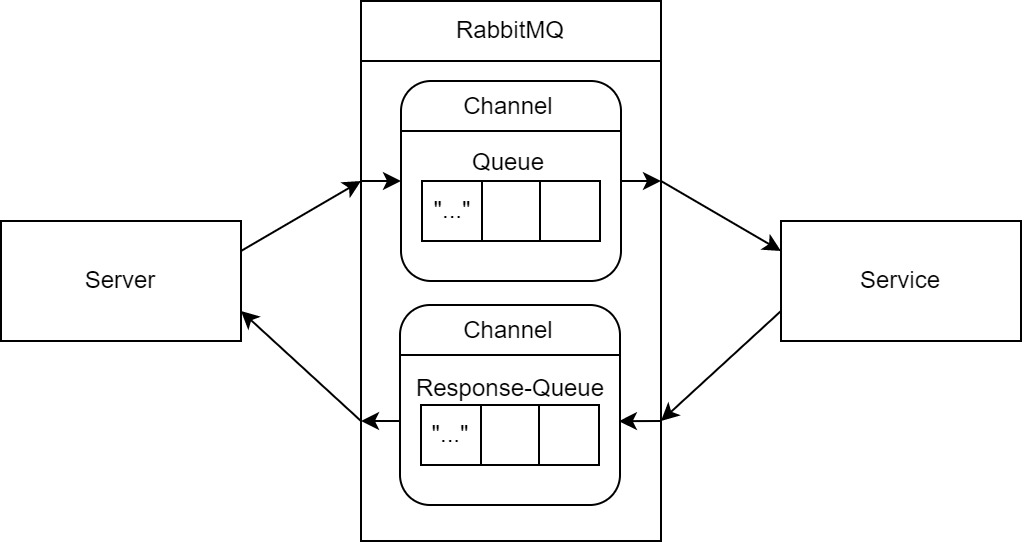
\includegraphics[width = 15cm]{bilder/Rabbit3}
    \caption{Kommunikation mit RabbitMQ}
\end{figure}

\subsubsection{Implementierung des KI-Services}
Der implementierte KI-Service lädt im ersten Schritt das KI-Modell, um mit diesem für jeden Eintrag in der Elasticsearch-Datenbank einen semantischen Vektor zu generieren. Dieser semantische Vektor wird ebenfalls in der Datenbank gespeichert und kann für zukünftige abfragen genutzt werden.
Nachdem sämtliche Einträge in der Elasticsearch-Datenbank indiziert wurden, beginnt die Programmablaufschleife. Der erste Schritt der Schleife ist das Warten auf eingehende Nachrichten. Diese Nachrichten werden über RabbitMQ aus der, für den Service definierten, Queue ausgelesen. Falls keine Anfrage an den Service eingetroffen ist, wartet der Dienst auf unbestimmte Zeit. Nach dem erfolgreichen Auslesen einer Nachricht, fängt der KI-Service an, die Anfrage zu bearbeiten. Im ersten Schritt wird aus dem Satz, den der Nutzer an den Service geschickt hat, ein semantischer Vektor generiert. Dazu wird das gleiche KI-Modell wie bei der Indizierung der Einträge in der Datenbank genutzt. Daraufhin nutzt der Service den generierten Vektor und die \texttt{cosineSimilarity()} Funktion der Elasticsearch, um die semantisch ähnlichsten Texte aus der Datenbank herauszufiltern. Die Anzahl der gelieferten Ergebnisse ist abhängig von den übergebenen Parametern. Der Nutzer kann im Frontend das Key-Value-Paar \texttt{search\_{}size} eingeben, welches in der Anfrage an den Service mitgeliefert wird. Sollte der Nutzer beispielsweise \texttt{\glqq search\_{}size : 3\grqq{}} eingeben, so werden die drei ähnlichsten Artikel zur gestellten Anfrage zurückgegeben. Die Ergebnisse werden in die Response-Queue des Services geschrieben, damit sie im Backend weiter verarbeitet werden können. Nach erfolgreichem Durchlaufen des Prozesses, geht der Service wieder zum Zustand \glqq Auf Anfrage warten\grqq{} über. Veranschaulicht wird der Programmablauf des Services in Abbildung 13.

\begin{figure}[H]
  \centering
    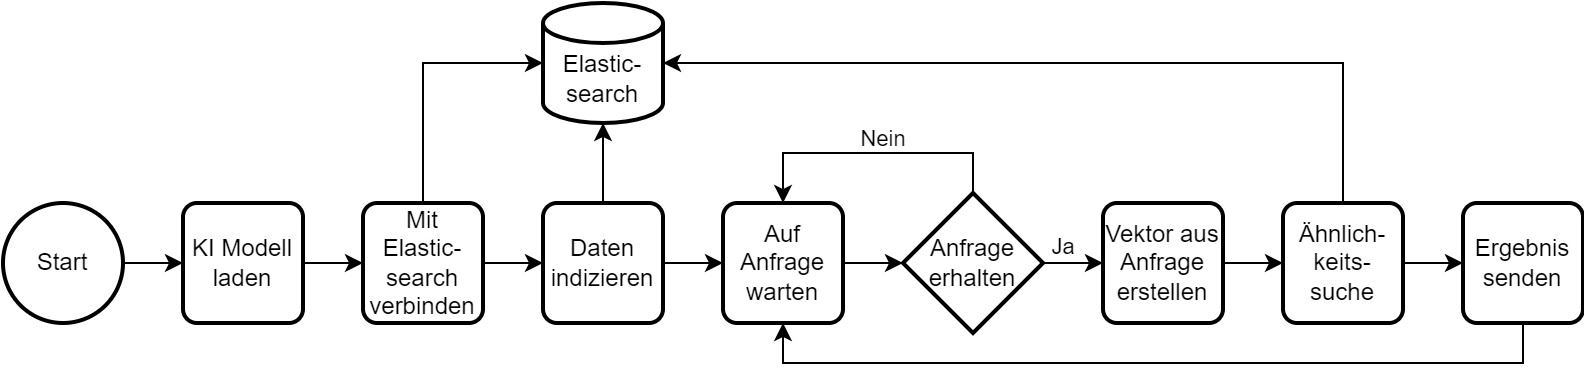
\includegraphics[width = 15cm]{bilder/KIAblauf}
    \caption{Ablaufdiagramm der Textähnlichkeitssuche}
\end{figure}

Damit der KI-Service eine Textähnlichkeitssuche durchführen kann, muss zunächst das BERT Modell importiert werden. Dieses kann der Service beim Starten automatisch aus dem offiziellen Tensorflow-Hub herunterladen. Anschließen wird eine Tensorflow-Session erstellt und gestartet. 

\begin{lstlisting}[language=Python, caption={Laden des BERT-Modells}]
embed = hub.Module("https://tfhub.dev/google/universal-sentence-encoder/2")
\end{lstlisting}

Im zweiten Schritt verbindet sich der Service mit der Elasticsearch-Datenbank. Dazu wird die URL, unter der die Elasticsearch erreichbar ist aus den Environment-Variablen geladen. Die Environment-Variablen können entweder beim manuellen Starten des Services mitgegeben werden oder falls der Service mit Docker gestartet wird, in der Docker-Compose File definiert werden. Mithilfe der URL initialisiert der Service eine Elasticsearch-Instanz und speichert sie in der Variable \texttt{client} ab. 

\begin{lstlisting}[language=Python, caption={Starten der Elasticsearch-Instanz}]
elasticsearch_url = os.environ.get('ELASTIC_URL')
client = Elasticsearch(elasticsearch_url)
\end{lstlisting}

Nachdem sich der Service erfolgreich mit der Elasticsearch verbunden hat, beginnt das Indizieren der Daten in der Datenbank. Dazu wird die Methode \texttt{index\_{}data()} aufgerufen. Der Datensatz, der für den Prototyp verwendet wurde, ist ein Auszug aus den gestellten Fragen im Forum Stackoverflow. In dem Datensatz sind 18.600 Fragen vorhanden. Jede Frage besteht aus einem Titel und einem Body. In einem Fragen-Body ist eine genauere Erläuterung der Frage, mit eventuellen Codeausschnitten oder Verlinkungen. Für die Indizierung ist lediglich der Titel der Frage genutzt worden. Das bedeutet im Umkehrschluss, dass der Titel der Frage repräsentativ für die gesamte Frage stehen muss. Nach Möglichkeit soll der Titel den gesamten Inhalt der Frage kurz und bündig zusammenfassen. Aus diesem Grund eignet Stackoverflow sich besonders gut für den Datensatz, da in den Guidelines \glqq Write a title that summarizes the specific problem\grqq{} explizit erwähnt wird.\footcite{stackoverflow2022question}

Nach erfolgreicher Indizierung sämtlicher Fragestellungen geht der Service in die Programmablaufschleife über. Die Schleife beginnt mit der Initialisierung der RabbitMQ-Verbindung. Dort verbindet sich der der Textähnlichkeitsservice mit der Queue \texttt{text-similarity}. Bei einer eingehenden Anfrage ruft die \texttt{callback} Funktion die \texttt{respond} Funktion auf, die den KI-Algorithmus aufruft und sich um die Verarbeitung der Antwort kümmert. Die Funktion \texttt{handle\_{}query()} benötigt als Parameter die Query die vom Nutzer gestellt wurde und die Anzahl der Ergebnisse, die zurückgegeben werden sollen. Beide Parameter werden aus aus der Anfrage, die über RabbitMQ an den Service gesendet wurde, ausgelesen. Sollte es vorkommen, dass der Nutzer keine \texttt{search\_{}size} angegeben hat, wird der Standartwert 1 gesetzt.
 
\begin{lstlisting}[language=Python, caption={Auslesen der search\_{}size und Ausführen der KI}]
search_size = 1
    for p in params:
        if "search_size" in p.values():
            search_size = p["value"]

    message = handle_query(query, search_size)
\end{lstlisting}

Innerhalb der \texttt{handle\_{}query()} Methode wird zunächst der Satz, der vom Nutzer gesendet wurde, durch die Methode \texttt{embed\_{}text()} in einen Vektor konvertiert. Dieser wird anschließend in das Feld \texttt{\glqq params\grqq{}} in der Such-Query für die Elasticsearch geschrieben. In dem Feld \texttt{\glqq source\grqq{}} wird die Ähnlichkeitsanalyse definiert. Die Elasticsearch implementiert die Funktion \texttt{cosineSimilarity()}, die zwei Vektoren als Parameter annimmt. Der erste Vektor ist der  aus der Query zuvor generierte Vektor. Der zweite Vektor ist der aus dem Titel der Frage generierte Vektor. 

Mit der \texttt{client.search()} stellt der Service die Anfrage an die Elasticsearch mit der zuvor definierten Query. In der Anfrage wird über das Feld \texttt{\glqq size\grqq} die Anzahl der gewünschten Ergebnisse mitgeliefert. Wenn die \texttt{search\_{}size} beispielsweise 3 beträgt, werden die drei Fragen mit den ähnlichsten Vektoren in die Variable \texttt{response} geschrieben. Im nachfolgen Codesegment sind die zuvor beschriebene Erstellung des Query Vektors, der Such-Query für die Elasticsearch und die Anfrage an die Elasticsearch dargestellt.

\begin{lstlisting}[language=Python, caption={Ähnlichkeitssuche in der Elasticsearch}]
query_vector = embed_text([query])[0]
script_query = {
    [...]
        "source": "cosineSimilarity(params.query_vector, doc['title_vector']) + 1.0",
        "params": {"query_vector": query_vector}  
}
response = client.search(
    [...]
        body={
            "size": search_size,
            "query": script_query,
            [...]
        }
)
\end{lstlisting}

Die Response der Elasticsearch wird nach erfolgreicher Durchführung wieder an die \texttt{respond} Funktion übergeben. Dort wird die Nachricht vorbereitet, die als Response auf die Anfrage vom Backend zurückgesendet wird. Die Antwort wird an RabbitMQ in die Queue \texttt{response-text-similarity} gesendet.

Der Schleifendurchlauf des Services ist damit abgeschlossen. Der Service geht nun wieder, wie in Abbildung 13 zu sehen, zum Zustand \glqq Auf Anfrage warten\grqq{} über. 

\subsubsection{Management der Services}
Die entworfene Softwarearchitektur unterstützt eine beliebige Anzahl an KI-Services. Die Services, die über das System erreichbar sein sollen, müssen über die API registriert werden. Jeder Service implementiert eine Verbindung zur RabbitMQ Schnittstelle, damit die Anfragen und Antworten asynchron zwischen dem Backend und dem jeweiligen Service gesendet werden können. Eine der Kernanforderungen für eine Architektur, die austauschbare KI-Services unterstützt, ist die dynamische Registrierung und Deregistrierung. Eine Registrierung beschreibt das Hinzufügen eines neuen Services im System, ohne den Quellcode anpassen zu müssen. Um dies zu ermöglichen, braucht es einen persistenten Speicher, in dem die zur Verfügung stehenden Services aufgelistet sind. Zur persistenten Speicherung von kleineren Datenmengen, eignet sich eine MySQL-Datenbank. Innerhalb der Datenbank werden die aktiven Services in der Tabelle \texttt{services} abgespeichert. Zu jedem Service gibt es einen Namen mit der Bezeichnung \texttt{service} und einen Anzeigenamen mit der Bezeichnung \texttt{display\_{}name}. Der Name wird für das interne Routing über RabbitMQ genutzt. Der Anzeigename wird im Frontend innerhalb des Dropdowns für die Auswahl des Services verwendet.

\subsubsection{Automatisierte Transformation des Inputs}
Bei der Nutzung eines KI-Services kann es dazu kommen, dass die Eingaben in einer bestimmten Form vorliegen müssen. Dies ist besonders dann von Bedeutung, wenn Künstliche Intelligenzen von Drittanbietern verwendet werden. Da die Implementation oftmals als Blackbox erfolgt und nur eine Schnittstelle nach außen bereitgestellt wird, kann nicht der Algorithmus an die Daten angepasst werden, sondern die Form der Daten muss an den Algorithmus angepasst werden. Daten kommen jedoch häufiger mit überschüssigen Informationen, je nach Quelle und Methode der Datenerhebung. Die Bereinigung per Hand ist sehr aufwändig und führt schnell zu Fehlern. Sollten Echtzeitdaten an einen KI-Service angeschlossen werden, ist eine händische Bereinigung grundsätzlich nicht möglich.

Um diesem Problem entgegenzuwirken, wurde im Backend ein Algorithmus entwickelt, der Daten mithilfe einer Transformationsanleitung automatisch bereinigen kann. Die Transformationsanleitung wird durch den Anwender eingegeben und hat folgende Form:

\begin{lstlisting}[language=Python, caption={Beispiel einer Transformationsanleitung}]
{
  "seperator": "\n",
  "replace": [
    {
      "old":"\[(\d*:?)*\]",
      "new":""
    }
  ]
}
\end{lstlisting}

Aktuell im Prototyp unterstützte Transformationsoperationen sind \texttt{sperator} und \texttt{replace}. Der \texttt{sperator} teilt die vom Nutzer eingegebene Query in mehrere einzelne Queries auf. Dazu nutzt er die \texttt{split} Operation aus Python, die für Strings standardmäßig verfügbar ist. In der Transformationsanleitung wird ebenfalls ein Array an \texttt{replace} Operationen angegeben. Jeder Eintrag im \texttt{replace} Array enthält ein Objekt mit Key-Value Paaren \texttt{old} und \texttt{new}. Der alte String wird durch den neuen String ersetzt. Dazu wird die \texttt{replace} Funktion aus dem Python Package \texttt{re} verwendet. Die \texttt{replace} Funktion nutzt Regular-Expression als Syntax für das Ersetzen. Dadurch sind auch komplexere Ersetzungsverfahren möglich. Im Beispiel für eine Transformationsanleitung wurde eine Regular-Expression zur Entfernung eines Zeitstempels mit der Form \texttt{[12:25:10]} angegeben. Der nachfolgende Code zeigt die Implementierung der \texttt{transform} Methode, die mithilfe der Anleitung die Transformation durchführt. Zunächst wird die Query in einzelne Nachrichten geteilt. Anschließend läuft eine Schleife über sämtliche Nachrichten und wendet die Transformationsschritte an. Der Algorithmus gibt ein Array an transformierten Nachrichten zurück.

\begin{lstlisting}[language=Python, caption={Transformationsalgorithmus}]
def transform(file: str, transform_json):
    [...]
    parts = file.split(transform_json['seperator'])
    messages = []
    for m in parts:
        for replacer in transform_json['replace']:
            m = re.sub(replacer['old'].replace("\\\\", "\\"), replacer['new'], m)
        m = m.strip()
        messages.append(m)
    return messages

\end{lstlisting}

\subsubsection{Fehlerbehandlung}
Während der Laufzeit des Programms kann es dazu kommen, dass im vom Nutzer produzierte Fehler auftreten. Der Nutzer kann im Bereich der Transformation syntaktisch nicht korrekte Texte eingeben, die Backend verarbeitet werden. Da Nutzereingaben ohne weitere Behandlung ebenfalls ein Sicherheitsrisiko für die Infrastruktur darstellen können, wird im Backend ein System implementiert, um die Verarbeitung der Eingaben in einer isolierten Umgebung ausführen zu können. Ähnlich wie bei der Verifizierung des JWT, ist das System zur Fehlerbehandlung auch mit Function-Wrappern und Annotations umgesetzt. 

Im Backend wird ein Exception-Handler definiert der eine Funktion mit zuvor übergebenen Parametern ausführt. Da eine fehlerhafte Ausführung auch dort zum Programmabsturz führen würde, wird die Funktion in einem Try-Except Block gekapselt. Die innerhalb dieses Blocks auftretenden Fehler werden abgefangen und in einem Exception-Objekt gespeichert. Innerhalb des Exception-Objekts ist die produzierte Fehlermeldung gespeichert. Über \texttt{str(e)} kann auf die Fehlermeldung zugegriffen werden. Innerhalb des Except-Blocks wird die Fehlermeldung an den Logger weitergegeben, um diese in einer Datenbank persistent zu speichern. Nach erfolgreichem Log wird dem Frontend in einer HTTP-Response der Statuscode 500 \glqq Internal Server Error\grqq{} zurückgegeben.\footcite{fielding1999rfc2616}

\begin{lstlisting}[language=Python, caption={Exception-Handling mithilfe von Wrappern}]
[...]
 @wraps(f)
        def decorator(*args, **kwargs):
            try:
                return f(*args, **kwargs)
            except Exception as e:
                logger.log("error", f"[Server, {msg}]: {str(e)}", "none")
                return r.respond({"success": False, "error": str(e)}, status=500)
            [...]
\end{lstlisting}

Jede Funktion, die in innerhalb des Exception-Handlers ausgeführt werden soll, wird mit der Annotation \texttt{@exception\_{}handler("...")} versehen. Innerhalb des Parameters wird der Ort, an dem die Funktion ausgeführt wird, und damit der Fehler auftritt, als String übergeben. Diese Information wird genutzt, um innerhalb des Fehlerlogs den Ort des Fehlers aufzulisten.

\subsubsection{Event Logging}
Das Backend implementiert ein Event-Logging-System mit dem Zustände und Informationen des Systems in einer Datenbank gespeichert werden können. Mithilfe von Logs können Entwickler den Ablauf eines Programms besser nachvollziehen und auftretende Fehler schneller zu ihrer Quelle zurückverfolgen. Es ist ebenfalls möglich, Systeme aufzusetzen, die die auf Logs auslesen und beim Auftreten eines Errors die zuständigen Personen alarmieren. Eine Herausforderung bei einem Logging System ist es, dass das System beim Entwickler durch das Loggen keinen erheblichen Mehraufwand produzieren soll. Im Backend wurde ein Logging System entwickelt, welches mit einer einzigen Funktion angesteuert werden kann. Die Log Funktions des Loggers wird in den verschiedenen Bereichen der Anwendung über \texttt{from logs.logger import log} importiert. Nach erfolgreichem Import, steht die \texttt{log} Funktion zur Verfügung. 

Für einen Log müssen drei Parameter übergeben werden, der Log Level, eine Message und die UUID. Die möglichen Ausdrücke für die Log Level sind in Tabelle 4 aufgeführt. Die unterstützten Log Level leiten sich aus der Funktionalität von Grafana ab, welche diese Logs mit einer zugeordneten Farbe visualisiert.

\begin{table}[H]
\centering
\begin{tabular}{c|c|c}
\textbf{Ausdruck} & \textbf{Log Level} & \textbf{Farbe}\\
\hline
emerg & critical & lila\\
fatal & critical & lila\\
alert & critical & lila\\
crit & critical & lila\\
critical & critical & lila\\
err & error & rot\\
eror & error & rot\\
error & error & rot\\
warn & warning & gelb\\
warning & warning & gelb\\
info & info & grün\\
information & info & grün\\
notice & info & grün\\
dbug & debug & blau\\
debug & debug & blau\\
trace & trace & hellblau\\
* & unknown & grau
\end{tabular}
\caption{Log Level des Event Logging Systems}
\end{table}

Innerhalb der Log Funktion wird eine Datenbank-Query mit den drei Parametern und einem aktuellen Zeitstempel erstellt. Der Zeitstempel kann mithilfe des \texttt{datetime} Packages erstellt werden. Über \texttt{cursor.execute()} wird die erstellte Query in der MySQL-Datenbank ausgeführt. Der Log wird als Eintrag in der Tabelle \texttt{logs} gespeichert. Im folgenden Codeausschnitt ist die Log Funktion abgebildet.

\begin{lstlisting}[language=Python, caption={Erstellung eines Logs}]
def log(level, message, uid):
    [...]
    query = f"INSERT INTO logs (`level`, `message`, `timestamp`, `uid`) VALUES (%s, %s, %s, %s)"
    cursor.execute(query, (level, message, datetime.utcnow(), str(uid)))
    [...]
\end{lstlisting}

Die produzierten Logs, die in der MySQL-Datenbank hinterlegt werden, können in Grafana visualisiert werden. Dazu muss ein Dashboard angelegt werden. Innerhalb des Dashboards wird ein durch Grafana bereitgestelltes Logs-Panel benötigt. Grafana ordnet die anzuzeigenden Daten grundsätzlich nach dem Zeitpunkt der Erstellung. Innerhalb des Logs-Panels wird der aktuellste Log oben angezeigt, die anderen chronologisch absteigend. Da in Grafana die MySQL-Datenbank als Datenquelle hinterlegt ist, muss auch die Abfrage der Daten ist SQL stattfinden. Innerhalb der SQL Abfrage ist die Auswahl des timestamps an erster Stelle durch Grafana vorgegeben. Weitere Spalten können beliebig gewählt werden. Eine Spalte mit dem Namen \glqq message\grqq{} wird direkt im Logs-Panel angezeigt, ohne den jeweiligen Log ausklappen zu müssen. Der Name \glqq level\grqq{} ist ebenfalls von Grafana reserviert. Sollte sich der Eintrag der \glqq level\grqq{} Spalte mit einem der Ausdrücke aus Tabelle 3 decken, so wird die entsprechende Farbe für den Log genutzt. Weitere selektierte Spalten werden durch Ausklappen des jeweiligen Log-Eintrags sichtbar. Die genutzte Query zur Abfrage der Logs ist im nachfolgenden Codesegment dargestellt.

\begin{lstlisting}[language=SQL, caption={Query zur Abfrage der Logs in Grafana}]
SELECT timestamp, message, level, uid from db_logs.logs;
\end{lstlisting}

Das Log Panel mit den aus der Query resultierenden Logs ist in Abbildung 14 abgebildet.

\begin{figure}[H]
  \centering
    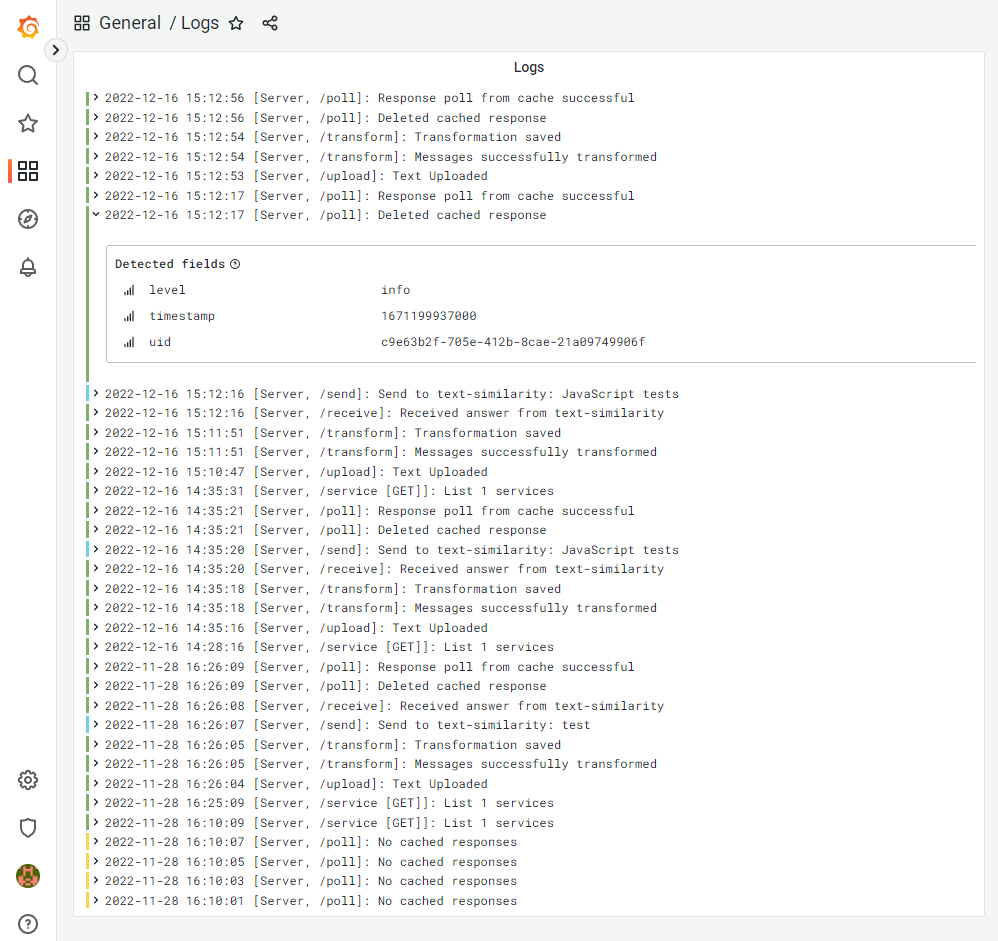
\includegraphics[width = 15cm]{bilder/grafana}
    \caption{Logs in Grafana}
\end{figure}

\subsubsection{Website mit Angular}
Damit ein Anwender die Schnittstelle zur Anbindung von Daten an KI-Services nutzen kann, wurde eine Website entworfen und entwickelt. Die grundlegende Funktionsweise der Website ist in den Abschnitten 4.1 Anforderungen und 4.2 Konzeption beschrieben. In diesem Kapitel liegt der Fokus auf der technischen Umsetzung der Website. 

Das Frontend wurde mit dem Framework Angular entwickelt. In Abbildung 15 ist der fertiggestellte Prototyp der Website dargestellt. 

\begin{figure}[H]
  \centering
    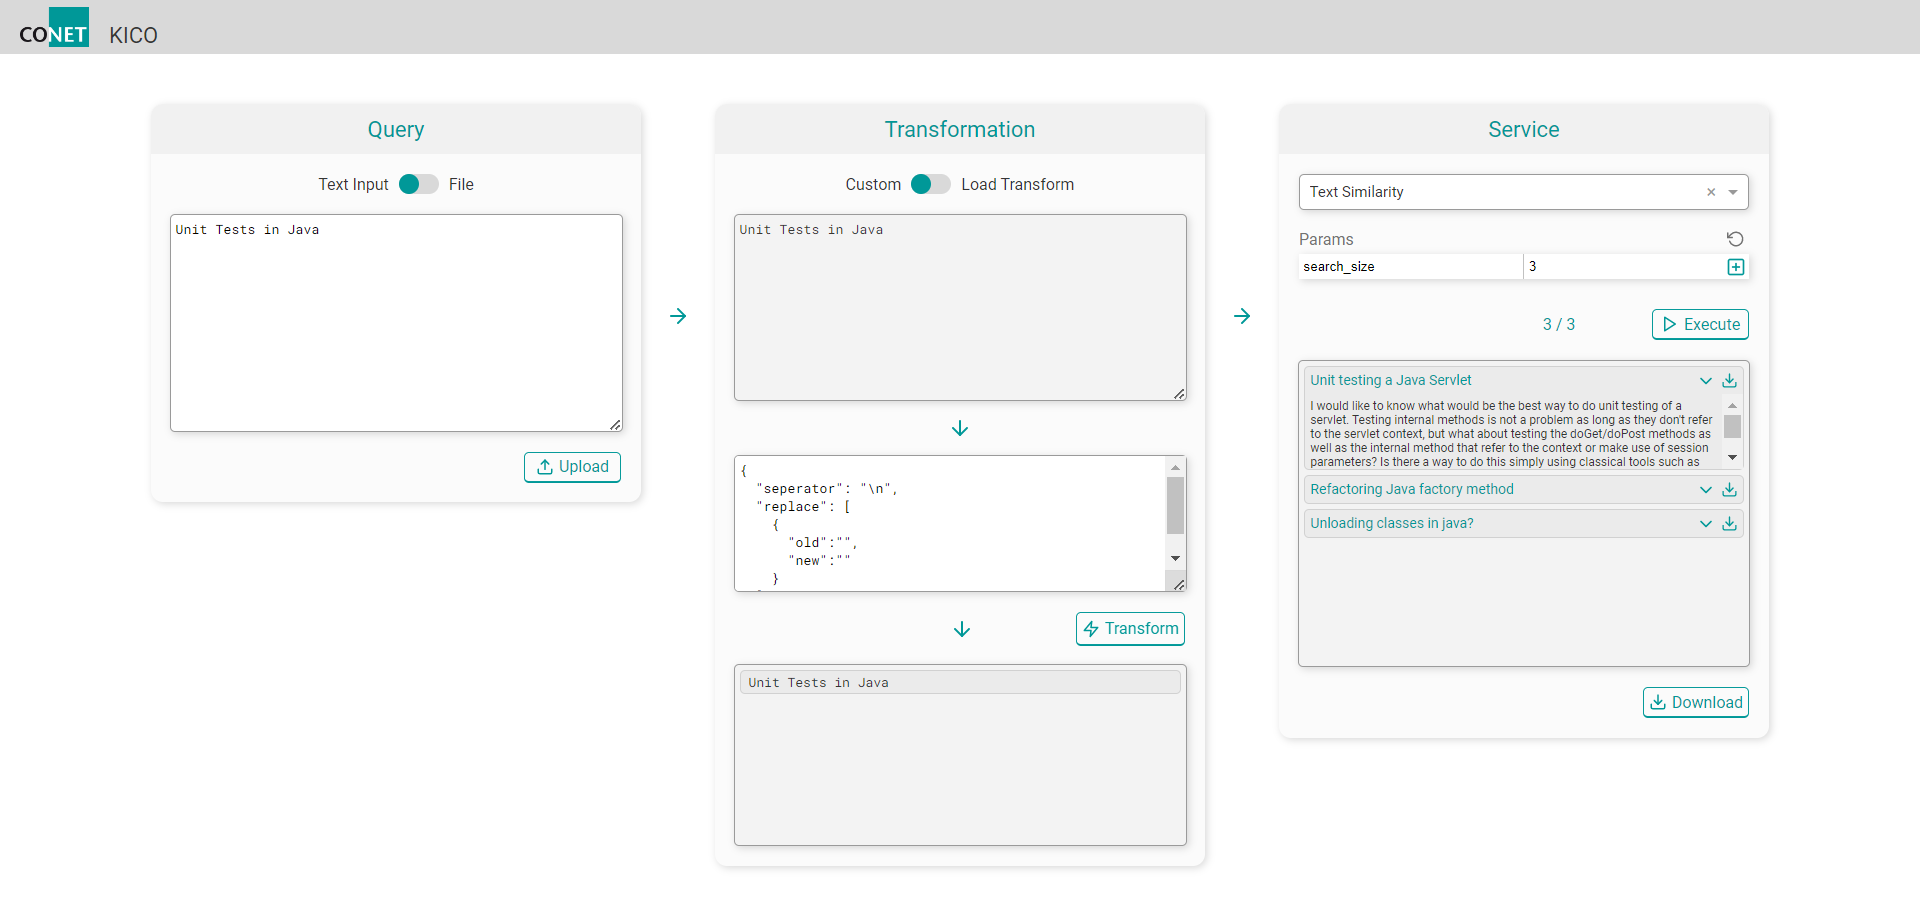
\includegraphics[width = 15cm]{bilder/website}
    \caption{Gesamtansicht der Website}
\end{figure}

Wie in den Anforderungen beschrieben, teilt sich die Website in drei Bereiche auf. In Angular ist es möglich, eigene Components zu definieren. Ein Component besteht aus drei Dateien. Die grundlegende Datei ist eine TypeScript Datei. Innerhalb dieser Datei wird der eigentliche Component definiert. Zunächst muss dafür \texttt{Component} aus \texttt{@anuglar/core} importiert werden. Im Anschluss im Bereich unter \texttt{@Component} ein selector, eine templateUrl und die styleUrls definiert. Der selector beschreibt, wie der Component im HTML Code aufgerufen werden soll. Jeder Component braucht einen individuellen Namen. Um die eigenen Components von den Components, die durch Angular bereitgestellt sind, unterscheiden zu können, befindet sich zu Beginn jedes Namens das Prefix \texttt{app-}. Die templateUrl gibt den Pfad der dazugehörigen HTML Datei an. Diese Datei ist die zweite Datei, die zur Erstellung eines Components notwendig ist. Innerhalb der styleUrls können mehrere Pfade zu verschiedenen Dateien angegeben werden. Die SCSS-Datei ist die dritte Datei, die zur Erstellung eines Component benötigt wird. Im folgenden Codeausschnitt ist die Initialisierung des Query-Imput-Components innerhalb der TypeScript-Datei dargestellt.

\begin{lstlisting}[language=Python, caption={Definition eines Components}]
import { Component, OnInit } from '@angular/core';

@Component({
  selector: 'app-datasource-input',
  templateUrl: './datasource.input.component.html',
  styleUrls: ['./datasource.input.component.scss']
})
\end{lstlisting}

Innerhalb der TypeScript-Datei können Variablen und Funktionen definiert werden. Diese können dazu genutzt werden, Nutzerinteraktionen mit der Website festzuhalten, oder Ereignisse darzustellen. In der Query-Input-Component wird die Variable \texttt{inputStr} definiert. Innerhalb dieser Variable wird die Eingabe, die der Nutzer im Textfeld der Query-Kachel tätigt, gespeichert. Für sich alleinstehend, hat die Variable jedoch keine Funktion. Diese bekommt sie erst durch den Code aus der HTML Datei. 

\begin{lstlisting}[language=Python, caption={Erstellung einer Textarea innerhalb der HTML-Datei}]
<textarea [(ngModel)]="inputStr" placeholder="Input..." class="text-input"></textarea>
\end{lstlisting}

Innerhalb der HTML Datei für die Query ist eine Textarea definiert. Über den Selector \texttt{[(ngModel)]} kann eine Variable angegeben werden, die mit dem Inhalt der Textarea synchronisiert wird. Sobald der Nutzer eine Eingabe in der Textarea tätigt, wird diese sofort in der TypeScript-Datei aktualisiert. 

Es ist ebenfalls ein \texttt{class} Attribut innerhalb der Textarea angegeben. Dieses setzt eine CSS Klasse für die Textarea. In der Definition der Component ist eine SCSS-Datei angegeben, die in diesem Schritt aufgerufen wird. Dort wird die Klasse \texttt{text-input} definiert und mit verschiedenen Style-Eigenschaften versehen. Diese Eigenschaften werden auf die Textarea angewandt.  

\begin{lstlisting}[caption={Style-Definition innerhalb einer SCSS-Datei}]
.text-input{
  border-radius: 5px;
  border: 1px solid #9A9A9A;
  box-shadow: 2px 2px 8px rgba(0,0,0,.15);
  resize: vertical;
  height: 206px;
  width: 90%;
  font-family: "Roboto Mono", sans-serif;
  padding: 5px;
}
\end{lstlisting}

Die daraus resultierende Textarea innerhalb der \glqq Query\grqq{} Kachel, ist in Abbildung 16 dargestellt.

\begin{figure}[H]
  \centering
    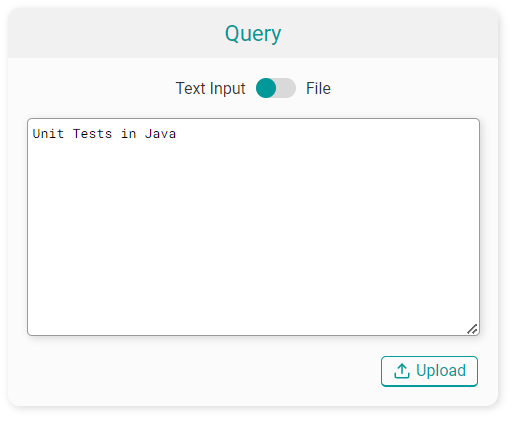
\includegraphics[width = 10cm]{bilder/websiteQuery}
    \caption{Query Kachel im Frontend}
\end{figure}

Der Bereich der Transformation besteht aus mehreren Sub-Components. Die obere und mittlere Textarea ist analog zu der Textarea aus der Query implementiert. Da die obere Textarea jedoch ausschließlich zur Bestätigung der Eingabe dient und nicht selbst zu Eingabe genutzt werden soll, wurde bei der Definition das Attribut \texttt{readonly} mitgegeben. Der untere Bereich der Transformation-Component teilt sich in zwei Components auf. Der übergeordnete Component ist das \texttt{transformation.result}. Dies ist die graue Box, in der eine Liste an transformierten Eingaben dargestellt werden. Jedes Element der Liste ist ein \texttt{transformation.result.item} Component. In Angular kann eine Liste im HTML-Code direkt aus einer Variable erzeugt werden. Dazu wird \texttt{*ngFor} verwendet. Innerhalb der Schleife ist eine Variable aus der zugehörigen TypeScript-Datei angegeben, über die iteriert wird. Sollte sich die Variable zur Laufzeit ändern, so wird auch direkt die HTML Datei angepasst. Der folgende Codeausschnitt zeigt die Implementierung des \texttt{transformation.result} Components.

\begin{lstlisting}[language=Python, caption={Anzeige der Results aus der Transformation}]
<div class="container">
  <li *ngFor="let item of results; index as i" class="list-results">
    <app-transformation-result-item [text]="item"></app-transformation-result-item>
  </li>
</div>
\end{lstlisting}

In Abbildung 17 ist die Transformation der Query, sowie das Ergebnis abgebildet.

\begin{figure}[H]
  \centering
    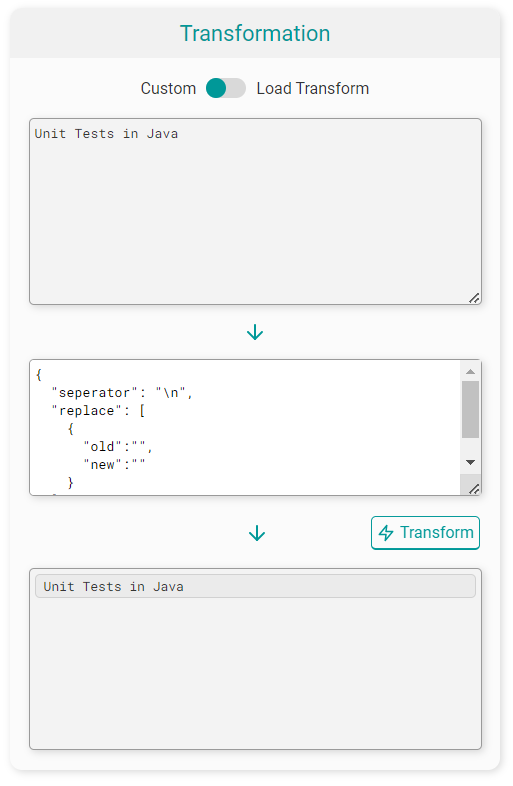
\includegraphics[width = 8cm]{bilder/websiteTransformation}
    \caption{Transformation Kachel im Frontend}
\end{figure}

Der dritte Bereich der Website stellt die Auswahl und Ergebnisauflistung des KI-Services dar. Zur Datenakquirierung werden in Angular-Services verwendet. Diese sind TypeScript-Dateien, die Kommunikation zur API regeln. Eine der Funktionen aus dem Service für die Service-Component ist \texttt{getService()} Methode. 

\begin{lstlisting}[language=Python, caption={Abfrage der Services}]
getServices() {
  const headers = {'Authorization': environment.token}
  return this.http.get<any>(environment.backend_url + '/service', {headers})
}
\end{lstlisting}

Diese kann innerhalb der TypeScript-Datei der Component aufgerufen werden. Die \texttt{getService()} Methode stellt einen HTTP-GET-Request an die \texttt{/service} Route der API. Die genaue URL der API wird aus den Environmentvariablen ausgelesen. Die Methode gibt jedoch nicht direkt die Response auf den Request zurück, sondern ein Objekt vom Typ Observable. Innerhalb des TypeScript-Datei des Components kann auf dieses Observable subscribed werden. Durch diese Herangehensweise wird ein asynchroner Aufruf an die API gesendet und bei einer Response das Ergebnis verarbeitet. Das Ergebnis ist hierbei eine Liste der verfügbaren KI-Services. Diese werden in der Variable \texttt{services} gespeichert.

\begin{lstlisting}[language=Python, caption={Subscriben auf einen Observable}]
this.serviceService.getServices().subscribe(res => {
  this.services = res['services']
})
\end{lstlisting}

Im HTML des Service-Components wird die Liste der Services für ein Dropdown verwendet. Eine weitere Funktion von Angular sind Events. Ein Event kann von einem Component ausgelöst werden. Innerhalb des Components, dass das untergeordnete Component implementiert, kann auf dieses Event reagiert werden. Es besteht die Möglichkeit TypeScript Code auszuführen oder vordefinierte Funktionen aufzurufen. Im Dropdown wird das \texttt{changeEvent} abgefangen. Dieses löst aus, wenn der Nutzer ein neues Element aus dem Dropdown ausgewählt hat. Dabei wird die Funktion \texttt{serviceSelected()} aufgerufen.

\begin{lstlisting}[language=Python, caption={Dropdown zur Auswahl der Services}]
<app-dropdown [elements]="services" (changeEvent)="serviceSelected($event)"></app-dropdown>
\end{lstlisting}

Die Tabelle für die Parameter nutzt ebenfalls \texttt{*ngFor}, um die einzelnen Reihen zu generieren. 

Der letzte Component innerhalb des Services ist der \texttt{service.result} Component. Dieser zeigt ein Ergebnis aus dem KI-Service an. Das Ergebnis besteht dabei aus einer Überschrift und einem Body. Damit die Ergebnisse beim Frontend eintreffen, muss der Nutzer nach der Auswahl des Services auf den Execute-Button klicken. Dadurch wird im Angular-Service die Methode \texttt{sendRequests()} aufgerufen, die dafür sorgt, dass die Anfrage für den KI-Service an die API gesendet wird. Anschließend wird die Funktion \texttt{pollResponses(expectedResponses: number)} mit der Anzahl der erwarteten Ergebnisse aufgerufen. Diese führt in einem 200ms Intervall die \texttt{poll()} Funktion aus, die eine Anfrage an die API stellt, ob bereits neue Ergebnisse des KI-Service im Backend zwischengespeichert wurden. Falls dies der Fall sein sollte, werden die Ergebnisse in der Response mitgeteilt und die Anzahl der erhaltenen Ergebnisse hochgezählt. Die Schleife läuft so lange, bis die Anzahl der erhaltenen Ergebnisse gleich der Anzahl der erwarteten Ergebnisse ist. Für jedes Ergebnis wird ein \texttt{service.result} Component in einer \texttt{*ngFor} Schleife erzeugt. Die Auflistung der Ergebnisse, sowie die zuvor beschriebenen Elemente der Service-Kachel, sind in Abbildung 18 zu sehen. 

\begin{figure}[H]
  \centering
    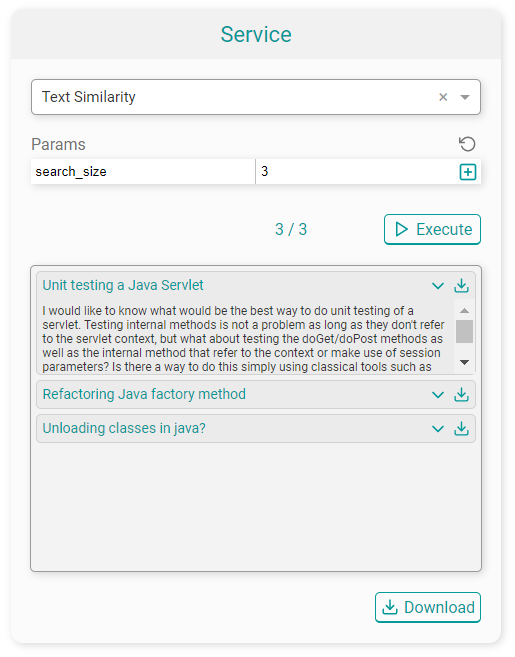
\includegraphics[width = 10cm]{bilder/websiteService}
    \caption{Service Kachel im Frontend}
\end{figure}

\subsection{Deployment der Software mit Docker}
Eine der Anforderungen von CONET war die plattformunabhängige Entwicklung der Schnittstelle. Aus diesem Grund wurden alle Bereiche der Softwarearchitektur über Docker-Container deploybar gemacht. Um eine eigens entwickelte Software in einen Container zu packen, muss zunächst ein Image aus der Software erstellt werden. Ein Image dient als Bauanleitung für den Container und enthält alle Dateien, die zur Ausführung des Programms benötigt werden. Ein Image kann über eine Docker-File generiert werden. Die Docker-File zur Erstellung des Images für das Backend ist nachfolgend abgebildet.

\begin{lstlisting}[language=Python, caption={Beispiel einer Dockefile}]
FROM python:3.10-slim
WORKDIR /app
ADD . /app
RUN pip install -r requirements.txt
EXPOSE 80
CMD ["python", "app.py"]
\end{lstlisting}

Innerhalb der Docker-File können Pakete aus dem Docker-Hub als Abhängigkeit angegeben werden, die beim Bauen des Images heruntergeladen werden. Im Falle des Backendes wird das Paket \texttt{python:3.10-slim} bezogen. Innerhalb der Dockerfile ist ebenfalls die Festlegung der Ordnerstruktur, sowie die Ausführung von Kommandos möglich.

Zum Bauen eines Images mithilfe der zuvor erstellten Docker-File wird der \texttt{build} Befehl benötigt. Für das Backend, den KI-Service, sowie das Frontend ist eine Docker-Compose-Datei zuständig. Die Docker-Compose-Datei kann in einer Linux- oder \ac{wsl}-Umgebung ausgeführt werden. Der dazu nötige Befehl lautet:
\begin{lstlisting}[caption={Build Befehl zur Erstellung von Docker-Images aus einer Compose-Datei}]
sudo docker compose -f '/path/to/compose/' build
\end{lstlisting}
Anschließend existieren drei Images in der Docker-Umgebung, die zum Bau der Container genutzt werden können. 

\begin{lstlisting}[caption={Docker-Compose-Datei zum Bauen der Docker-Images}]
version: '3.3'
services: 
    flask-backend:
        build: 
            context: ../BA-Backend/
            network: host
    flask-services:
        build:
            context: ../BA-Services/
            network: host
    frontend:
        build:
            context: ../BA-Frontend/
            network: host
\end{lstlisting}

Der nachfolgende Auszug aus der \texttt{docker-compose.core.yml} Datei zeigt die Bauanleitung für einen Container der MySQL-Datenbank. Innerhalb dieser Compose-Datei wird zunächst der Name des Services definiert. Unter diesem Namen ist der Docker-Container im Netzwerk durch andere Docker-Container erreichbar. Innerhalb des Services stehen mehrere Optionen zur Festlegung von Eigenschaften des Containers zur Verfügung. Über \texttt{ports} können ein oder mehrere Ports freigeschaltet werden, sodass der Container Zugriffe von außerhalb erlaubt. Im Bereich \texttt{volumes} stehen alle Ordner oder Dateien, die persistent gespeichert werden. Bei MySQL gibt es die Möglichkeit, ein initiales SQL-Skript anzugeben, welches nur bei der ersten Erstellung des Docker-Containers ausgeführt wird. Das SQL-Skript erstellt eine Datenbank und die benötigten Tabellen. Im \texttt{image} Bereich ist das Image zum Bauen des Containers angegeben. Dies ist entweder ein lokal vorhandenes oder ein im Docker-Hub angebotenes Image. Der letzte aufgeführte Punk \texttt{networks} beinhaltet das Netzwerk, in dem sich der Docker-Container befindet. Das Netzwerk wird benötigt, damit unterschiedliche Container miteinander kommunizieren können. Dazu muss sichergestellt werden, dass sämtliche Container im gleichen Netzwerk sind.

\begin{lstlisting}[caption={Docker-Compose-Datei zum Aufsetzen und Starten der Container}]
services:
    mysql: 
        ports: 
            - '3333:3306'
        volumes: 
            - mysql-conf:/etc/mysql/conf.d
            - mysql-storage:/var/lib/mysql
            - ./setup.sql:/docker-entrypoint-initdb.d/init.sql:r
        [...]
        image: mysql:latest
        networks:
            - custom-network
networks: 
    custom-network:
        driver: bridge
        name: custom-network
volumes:
    mysql-storage:
    mysql-conf:
\end{lstlisting}

Der Container kann mit folgendem Befehl gebaut und gestartet werden:
\begin{lstlisting}[caption={Starten eines Docker-Containers}]
sudo docker compose -f '/path/to/compose/' up -d
\end{lstlisting}

Sollte der Container anschließend wieder beendet werden, so wird folgender Befehl benötigt: 
\begin{lstlisting}[caption={Beenden eines Docker-Containers}]
sudo docker compose -f '/path/to/compose/' down
\end{lstlisting}